\chapter{Scheduling Part 1}

\section{Course information}
\paragraph{Groups.} The professor checked the spreadsheet of the groups uploaded by the deadline (last Friday). Student ID colours: \textbf{white}, enrolled, everything fine; \textbf{yellow}, in the list but with the \emph{career not active}: no problem for the project, but it must become active before the exam, or the exam cannot be recorded; \textbf{red}, \emph{not eligible} (e.g.\ attended the course for the first time two years ago). A one-person group is not acceptable: the project is practically impossible to complete alone. Students not yet in the spreadsheet must email the professor \textbf{by the end of the day} of the lecture, with their student ID and the group they want to join.

\paragraph{Assignment and grading.} The assignment is published, and correctly registered groups can start: a \textbf{loader} for the scratch-OS, so that programs are loaded at run time instead of being statically compiled into the OS image. Groups of \textbf{4 or fewer} have the basic requirements, groups of \textbf{5 or 6} also 3--4 additional ones; otherwise the projects are identical. The project is not complex, but the requirements document is long, since it tries to anticipate every question: read it carefully (about 5--6 hours) \emph{before} asking. Each requirement is worth the points stated in the assignment: the basic ones up to \textbf{14 points} for every group; the extra ones add nothing, but \textbf{missing} them \textbf{subtracts} points, so the basic requirements weigh the same in both versions.

\paragraph{Accounts.} When the groups are frozen (after the late registrations), each group gets an account and a repository on the lab's Git server, with the credentials sent by email. Students without a student ID yet can share a teammate's account (the password is random, so it can be shared safely). Nobody is evaluated on the number of contributions per account. \emph{Update:} the spreadsheet is now \textbf{frozen}: the accounts exist and the project can start; whoever emailed and got no answer should write again. Check your team composition: whoever registered with an old or temporary ID and now has a new one must email it, since each account is named after the current student ID and uses its student email. The Politecnico network was temporarily unreachable from outside, teaching-material servers included (reachable through the VPN); the material is published only on the professor's website, built on Git, not on the teaching portal.

\paragraph{Organisation.} From this week programming gets lighter and theory grows. This week and the next are on \textbf{scheduling}: the only implementation is the round-robin scheduler of the scratch-OS, in the second part of this lecture (Unit 2), the last difficult programming part of the course. No new code comes in the next lecture or next week, which leaves about two weeks to study it; the rest is theory and exercises on paper. One last week on the scratch-OS then adds a small synchronisation system call, and the second half of the course uses \textbf{FreeRTOS} from the \emph{user's} point of view: knowing how an OS works inside, we write application software on top of a real OS, very similar to the very limited scratch-OS but with much more, at a slightly higher level (with a simple exam exercise on it too). The labs start to include exam-like exercises on the first half of the course: next week's is on scheduling (some implementation, plus exam-style exercises in the optional part), the following one only exam-style exercises.

\section{Where we are}
The scratch-OS has system calls, privileged and unprivileged software, memory management and protection: since week 4 each task has its own RAM partition, and the MPU stops a task from touching memory that is not its own, so the kernel is safe from its tasks and the tasks from each other. But tasks still run \emph{one after the other}: B starts only when A has called \texttt{exit}, and while A waits one second between two lines the CPU is simply wasted. This week the kernel shares the CPU, and A and B run \emph{at the same time}. The units, in the same order in slides and notes:
\begin{itemize}
    \item \textbf{Unit 1, Process management: the ideas} (no code): tasks and their states, the task control block, when the scheduler runs, and three algorithms: first-come first-served, round robin and priority scheduling, compared on turnaround, waiting and response time with schedules solved on paper.
    \item \textbf{Unit 2, Context switch and round robin}: the preemptive round-robin scheduler prepared in the scratch-OS (task control block, context switch in the \texttt{PendSV} exception, SysTick-driven time slice, system calls that give the CPU away, idle task), observed with gdb, a different time slice and demo builds; then a hand-written \textbf{trace} that records every task switch and prints the schedule as a Gantt chart, like those drawn on paper in Unit 1.
    \item \textbf{Unit 3, Real-time basics}: tasks that must finish \textbf{on time}: hard, firm and soft deadlines; periodic, sporadic and aperiodic tasks; the notation (release, period, deadline, response time, lateness); utilisation and hyperperiod; \textbf{timeline scheduling} (the cyclic executive), built by hand and checked with the course tool \texttt{schedsim}.
\end{itemize}
\paragraph{Approach of the course.} There are many algorithms to study, but the \emph{mechanism} that runs any of them is always the same. So the scratch-OS implements \textbf{only one} (round robin): changing algorithm changes only a \emph{high-level} part of the OS, while the low-level mechanisms, above all the \textbf{context switch}, stay the same. An algorithm is a few lines of C, and implementing all of them would teach little; the context switch is much harder, and different on every machine. The implementation effort goes there; the other algorithms are studied in theory (and can be implemented as a personal exercise).

\section{Process management: the ideas}

\subsection{Program, process and task}
A \textbf{program} is code and data in memory, the result of compiling (e.g.\ the ELF file of our projects): by itself it does nothing. A \textbf{process} is a \emph{program in execution}: copied from FLASH to memory, with its kernel data structures created, and so on. It is the code (\textbf{text}) plus everything that changes while it runs: \textbf{data} (global and static variables), \textbf{stack} (local variables, arguments, return addresses) and \textbf{CPU state} (the PC, pointing at the next instruction, the SP and all the other registers). It runs \textbf{sequentially}: never two of its own instructions at the same time.

\paragraph{Process vs task.} Synonyms: general-purpose OSs (e.g.\ Linux books) talk about \emph{process management}, embedded OSs (e.g.\ FreeRTOS) about \emph{task management}. An embedded \textbf{task} has its own stack and CPU state, but usually \emph{no} private address space, open files or parent process: all tasks are linked into \textbf{one} program with the kernel. Week 4's A and B are tasks in exactly this sense: own code, stack and partition, in one executable.

\subsection{One CPU, several tasks}
A core executes one instruction stream at a time, so the tasks must share it: the kernel \textbf{interleaves} them (A, then B, then A again). Truly simultaneous execution is impossible on one core, but with short turns both seem to run together to a human; this is the simplest solution, and ours. Stopping A and starting B means saving A's whole CPU state (its \emph{context}) and loading B's: a \textbf{context switch}. Done correctly, A cannot tell it was stopped: it resumes at the same instruction with the same registers. The \textbf{scheduler} is the kernel part that decides which task runs next, following a \textbf{scheduling algorithm} (\textbf{policy}): e.g.\ each task runs 10\,ms, then gives the CPU to another; or each task runs to its end, then the next. Bachelor OS courses present the context switch as simple and abstract, but in practice it is complex because \textbf{machine-dependent}: it requires knowing exceptions, how a program is interrupted, how to move between privileged and unprivileged mode, and many other processor details. We implement it for the Cortex-M3; on an Intel processor it would be a completely different story.

The rest of the unit answers: what does the kernel know about each task? \emph{When} does the scheduler decide, and \emph{how}?

\subsection{Task states}
Only the kernel moves a task between \textbf{execution states}, which determine how the scheduler works. Even very simple OSs have \textbf{four} (complex ones such as Linux have more).

\begin{figure}[h]
\centering
\begin{tikzpicture}[
    state/.style={draw, rounded corners, minimum width=2.4cm, minimum height=0.9cm, font=\bfseries},
    >=Stealth, font=\small]
    \node[state] (run)     at (0,0)     {RUNNING};
    \node[state] (ready)   at (-3.5,-3) {READY};
    \node[state] (blocked) at (3.5,-3)  {BLOCKED};
    \node[state] (fin)     at (4.8,0)   {FINISHED};
    \node[font=\small\itshape] at (0,0.9) {one CPU: at most one task here};

    \draw[->] (ready) to[bend left=20] node[above left] {scheduler picks it} (run);
    \draw[->] (run) to[bend left=20] node[below right, align=center] {preempted\\or yield} (ready);
    \draw[->] (run) -- node[above] {exit} (fin);
    \draw[->] (run) to[bend left=20] node[right, align=left, xshift=2pt] {waits for an event\\(delay, data)} (blocked);
    \draw[->] (blocked) -- node[below] {event happens} (ready);
\end{tikzpicture}
\caption{Task states and transitions.}
\end{figure}

\begin{itemize}
    \item \textbf{RUNNING}: the task holds the CPU. On one core \emph{at most one} task is RUNNING; every other started task is in another state.
    \item \textbf{READY}: in memory with everything it needs except the CPU. The READY tasks are the ``bucket'' from which the scheduler takes the next task: the policy, implemented by an algorithm, decides which.
    \item \textbf{BLOCKED} (\textbf{waiting}): the task cannot run until an \emph{event} (a delay ends, data arrives, a resource is freed), so the CPU would be useless to it. E.g.\ during the scratch-OS's delay (sleep) the kernel parks the task here, which tells the scheduler not to give it the CPU. Whenever it gets control, the OS checks whether each blocked task's reason is gone (a task that sleeps 10\,ms must run again after 10\,ms). Any system call that behaviourally requires waiting blocks, not only delays (from a question in class): in Linux, reading or writing a file takes milliseconds while the CPU works at the micro/nanosecond scale, so a process calling \texttt{read} or \texttt{write} is BLOCKED until the disk (or other device) completes, usually signalling it with an interrupt, and then READY again. ``Blocked'' is a behavioural notion, not a hardware one.
    \item \textbf{FINISHED}: the task called \texttt{exit} (in the scratch-OS, the system call that tells the kernel the task is over) and never runs again. The OS knows the task is completed and can free the dynamic structures allocated for it; the scratch-OS has none, so for us this state does nothing more.
\end{itemize}
Transitions:
\begin{itemize}
    \item \textbf{READY $\to$ RUNNING}: the scheduler picks the task.
    \item \textbf{RUNNING $\to$ READY}: the kernel takes the CPU away (\textbf{preemption}) or the task gives it up (\textbf{yield}); either way it could still run.
    \item \textbf{RUNNING $\to$ BLOCKED}: the task asks to wait (a delay, data not yet available).
    \item \textbf{BLOCKED $\to$ READY}: the event happens. \textbf{Never straight to RUNNING}, in any OS: another task has the CPU, so the woken task waits its turn like every READY task, and the policy decides.
    \item \textbf{RUNNING $\to$ FINISHED}: the task calls \texttt{exit}.
\end{itemize}
With $N$ tasks on one CPU, at any moment exactly 1 is RUNNING, $M$ are BLOCKED and $N - M - 1$ READY (FINISHED ones aside). General-purpose systems also have a \textbf{NEW} state, for a process being created and not ready yet; our kernel creates all tasks at boot, before any runs, so it needs none. A scheduler is thus a \emph{policy}: a simple algorithm (a function) that knows all tasks and their states, uses this diagram to decide where each task goes, and picks the READY task that becomes RUNNING.

\subsection{What does a task look like?}
Scheduling needs assumptions on how tasks are written. A general-purpose OS lets a process be structured freely (as the tasks of the course project must be), but in the course OS a task has one of two structures: not just a simplification, but the assumption of \emph{every} embedded OS. (Most function names of this week come from FreeRTOS, which allows both, so they will look familiar later.) An embedded task is a C function that is:
\begin{itemize}
    \item \textbf{run to completion} (non-periodic task): setup, then the work, then exit to FINISHED (like week 4's task A); or
    \item an \textbf{endless loop} (periodic task\footnote{Here ``periodic'' is used informally, for a task that repeats its work forever. Unit 3 gives the precise definition of periodic, sporadic and aperiodic tasks.}): setup, then forever wait for an event, do the work, wait again (like week 4's task B). It never ends; this structure is very important, especially in real-time embedded systems.
\end{itemize}

\begin{lstlisting}[language=C]
/* Run to completion, like week 4's task A */
void task_a( void )
{
    setup();
    do_work();
    /* then return: the kernel calls exit for it */
}

/* Endless loop, like week 4's task B */
void task_b( void )
{
    setup();                 /* once, before the loop */
    for ( ;; )
    {
        wait_for_event();    /* e.g. "one second has passed": BLOCKED until then */
        do_work();
    }
}
\end{lstlisting}

Most embedded tasks are endless loops that never reach FINISHED, e.g.\ monitoring a sensor, read as long as the device is on: at each new reading the task wakes up, processes it and waits for the next. Waiting for an event needs OS support (very simple in our case), and it is what makes sharing work: a BLOCKED task leaves the CPU to the others, while a task that never waits (looping on busy work) keeps it as long as the kernel lets it.

\subsection{The task control block (TCB)}
With a scheduler, four run-time states and two task structures, the kernel needs a \textbf{data structure} per task, above all to save the full CPU context in memory when the task stops. Week 4's \texttt{struct task}, made to run two tasks, is extended to hold more: the \textbf{TCB} (\textbf{process control block}, PCB, in general-purpose systems), one record per task, so that the kernel can stop it and restart it later. It holds:
\begin{itemize}
    \item the \textbf{saved stack pointer}: where the task's registers were saved (pushed on its own stack) when it stopped; already in week 4's structure;
    \item the \textbf{state}: READY, RUNNING, BLOCKED or FINISHED; new, not in last week's code;
    \item the \textbf{identity}: name or number, entry function, stack and partition limits (mostly already in week 4's \texttt{struct task}). A name is not mandatory, but every OS has one: when debugging, a mnemonic name is much easier than a number;
    \item \textbf{scheduling information}: whatever the algorithm needs, e.g.\ a priority, or the wake-up time of a delayed task;
    \item a \textbf{link to the next TCB}, to build queues (e.g.\ of READY tasks).
\end{itemize}
A desktop OS's PCB holds much more: open files, memory maps, CPU time used, parent and children (Linux: \texttt{struct task\_struct}). In TCB terms, a context switch saves the CPU state, stores the SP in the old task's TCB, takes the SP from the new task's TCB and restores its CPU state. The TCBs live in a \textbf{static} structure such as an \textbf{array} (simple, but the set of tasks is fixed by its size) or a \textbf{dynamic} one such as a \textbf{linked list} (tasks added and removed at run time, each TCB pointing to the next); Linux organises almost every data structure with more than one element as a \emph{doubly} linked list (pointers to next and previous).

\subsection{When does the scheduler run?}
A very important point. Take two tasks and a scheduler that can interrupt one and run the other (whatever the policy). It runs at boot, to start the first task; afterwards, specific \textbf{events} activate it.

\begin{figure}[h]
\centering
\begin{tikzpicture}[x=0.95cm, y=0.8cm, font=\small]
    % row labels
    \node[left] at (0,2) {task A};
    \node[left] at (0,1) {task B};
    \node[left] at (0,0) {kernel};
    % task A
    \fill[gray!35] (0,1.7) rectangle (2,2.3);       \node at (1,2) {A runs};
    \fill[gray!35] (5,1.7) rectangle (8,2.3);       \node at (6.5,2) {A runs};
    \fill[gray!35] (11,1.7) rectangle (12.5,2.3);   \node at (11.75,2) {A runs};
    % task B
    \fill[gray!35] (2.5,0.7) rectangle (4.5,1.3);   \node at (3.5,1) {B runs};
    \fill[gray!35] (8.5,0.7) rectangle (10.5,1.3);  \node at (9.5,1) {B runs};
    \draw[pattern color=gray] (5,0.7) rectangle (6.5,1.3);
    \fill[gray!10] (5,0.7) rectangle (6.5,1.3);     \node at (5.75,1) {blocked};
    \draw[dashed] (6.5,0.7) rectangle (8,1.3);      \node at (7.25,1) {READY};
    % scheduler
    \foreach \x in {2,4.5,8,10.5} {
        \fill[black] (\x,-0.3) rectangle (\x+0.5,0.3);
        \node at (\x+0.25,-0.6) {\scriptsize sched};
    }
    % events
    \foreach \x/\lab in {2.25/timer tick, 4.75/blocking call, 8.25/yield, 10.75/exit} {
        \draw[dashed, gray] (\x,-0.3) -- (\x,2.6);
        \node[above] at (\x,2.6) {\lab};
    }
    % time axis
    \draw[->] (0,-1.1) -- (13,-1.1) node[right] {time};
\end{tikzpicture}
\caption{The four events that activate the scheduler: A's time slice ends (A: RUNNING $\to$ READY); B calls \texttt{delay} (B: RUNNING $\to$ BLOCKED); A gives up the CPU (A: RUNNING $\to$ READY); B finishes (B: RUNNING $\to$ FINISHED).}
\end{figure}

\textbf{The scheduler is not a task}: it is a kernel function, run only when an event calls it. The four \textbf{activation points}:
\begin{enumerate}
    \item \textbf{Timer tick}: a periodic hardware timer interrupt (\textbf{SysTick} on Cortex-M), in general \textbf{high-priority} (on Cortex-M a \emph{lower} number means a \emph{higher} priority).\footnote{In the scratch-OS of Unit 2, SysTick shares with PendSV the least urgent priority value used by the kernel, \texttt{0xE0}: the reason is explained there.} Every $x$ milliseconds, whatever runs is interrupted and the CPU enters the OS's interrupt service routine. This is how the OS gets time for its own work on a single core busy with programs (from a question in class): most of its work reacts to the tick, whose handler is a sequence of function calls, each an OS service; running the scheduler, to check whether another task should run, is one of them.
    \begin{itemize}
        \item Not mandatory, but the tick is \emph{the} place for a \textbf{preemptive} scheduler: even a task that will not release the CPU must give control to the OS (the ``brutal'' event: the task can do nothing about it).
        \item The \textbf{time slice} (\textbf{quantum}) is the longest a task may run before the scheduler is called; when it ends, the task can be preempted (RUNNING $\to$ READY).
        \item The tick also checks the BLOCKED tasks: one whose delay has ended goes BLOCKED $\to$ READY.
        \item It is the most complex activation point to implement: it requires knowing the hardware.
    \end{itemize}
    \item \textbf{Blocking call}: the running task makes a system call that waits (a delay, data not yet available, I/O to complete): RUNNING $\to$ BLOCKED, so another task must be chosen.
    \item \textbf{Yield}: the running task \emph{voluntarily} gives up the CPU, although it could continue (RUNNING $\to$ READY). Many OSs have a \texttt{yield} system call, in practice ``run the scheduler again'', e.g.\ after a task changed something in the system and wants the scheduler to reassess the best task to run.
    \item \textbf{Exit}: the running task finishes (RUNNING $\to$ FINISHED), and another must be chosen.
\end{enumerate}
Only the tick comes from outside: the other three are \textbf{system calls} of the running task. In the figure, B's delay ends while A runs: B is READY again but does \textbf{not} run, and the end of the delay does not by itself call the scheduler. A holds the only CPU, so the OS cannot take control before the next activation point (here A's yield; with a preemptive kernel, at the latest the next tick), and only then is it decided whether B runs.

\subsection{Preemptive vs cooperative}
A \textbf{preemptive} scheduler can take the CPU from a running task \emph{without its cooperation}, at any instruction, at a tick (or another interrupt), e.g.\ with the scheduler called in the timer tick. A \textbf{cooperative} one leaves it to the tasks to give control back: a task keeps the CPU until it blocks, yields or exits, and no tick switches tasks; e.g.\ no scheduler in the tick, but a \texttt{yield} system call that every task calls at some point. Week 4's scratch-OS is \emph{not} preemptive: the kernel regains control only at \texttt{exit}; SysTick is there, but its handler does nothing for scheduling, so A runs to its end, then B. \textbf{Interrupts are not preemption}: in a non-preemptive OS an interrupt (an external event) can still interrupt a task, but the scheduling question is whether the \emph{OS} can stop a task that has the CPU and give the CPU to another task; there, it cannot.
\begin{itemize}
    \item Cooperative is \textbf{simpler}: a task is never stopped in the middle of its work, so tasks interfere less.
    \item But it is \textbf{dangerous}: one task looping without blocking or yielding (e.g.\ stuck in an infinite loop) freezes the whole system, and a long task delays every urgent one.
    \item Preemptive keeps the system \textbf{responsive}, but a task can be stopped between any two instructions: \textbf{shared data needs protection}.
\end{itemize}
Likewise for algorithms: \textbf{non-preemptive} ones never take the CPU from a running task, \textbf{preemptive} ones do.

\subsection{Exercise: follow two tasks}
A preemptive kernel (every task gets a fixed time slice) runs tasks A and B; both are READY at boot. When a task becomes READY, it waits until the running task's time slice ends. Events, in order:
\begin{enumerate}
    \item the scheduler picks A;
    \item A calls \texttt{delay(10 ticks)};
    \item a tick ends B's time slice;
    \item A's 10 ticks have passed (the tick that detects it does not end B's slice);
    \item B's time slice ends;
    \item A calls \texttt{exit}.
\end{enumerate}
After each event, write the state of A and B and the transition that happened.

\paragraph{Solution.} At boot nothing distinguishes A and B: by the tie rule of all exercises \textbf{and of the exam}, the \textbf{lowest identifier} runs first (Section~\ref{w05:conventions}), so event 1 picks A.
\begin{center}
\begin{tabular}{l l l p{5.6cm}}
\hline
\textbf{after event} & \textbf{A} & \textbf{B} & \textbf{transition} \\
\hline
1. scheduler picks A & RUNNING & READY & A: READY $\to$ RUNNING \\
2. A calls delay & BLOCKED & RUNNING & A: RUNNING $\to$ BLOCKED, B: READY $\to$ RUNNING \\
3. B's slice ends & BLOCKED & RUNNING & none: no other task is READY, B keeps the CPU \\
4. A's delay is over & READY & RUNNING & A: BLOCKED $\to$ READY (not RUNNING: B's slice is not over) \\
5. B's slice ends & RUNNING & READY & B: RUNNING $\to$ READY (preempted), A: READY $\to$ RUNNING \\
6. A calls exit & FINISHED & RUNNING & A: RUNNING $\to$ FINISHED, B: READY $\to$ RUNNING \\
\hline
\end{tabular}
\end{center}

\begin{itemize}
    \item \textbf{Event 2}: \texttt{delay} blocks: A becomes BLOCKED, the scheduler runs, and B, the only READY task, starts.
    \item \textbf{Event 3}: B's time is over and the scheduler runs, but with A blocked it has no choice: B runs again. Preemption needs another READY task; otherwise the running task just continues, and the CPU does not idle waiting for A (implementing this correctly is not as easy as it sounds: see Unit 2).
    \item \textbf{Event 4}: A is READY, but B keeps its slice to the end: once given, a slice is not taken back, even if B already ran twice in a row.
    \item With A and B both BLOCKED, nothing could run, but the kernel must execute something anyway: Unit 2's answer is the \emph{idle task}.
\end{itemize}

\section{Scheduling criteria}
Policies are compared with \textbf{metrics}, which \textbf{conflict} (no algorithm is the best at all of them), so algorithms are usually compared on \textbf{averages} over all tasks. A task \textbf{arrives} (becomes READY) at $a$, needs $C$ units of CPU, \textbf{starts} for the first time at $s$ and \textbf{finishes} at $f$.
\begin{itemize}
    \item \textbf{CPU utilisation} (maximise): the fraction of time the CPU actually runs tasks; time in the scheduler, in other OS code or idle lowers it. The ideal 100\% is never reached: the closer, the better.
    \item \textbf{Throughput} (maximise): tasks finished per unit of time; the goal when finishing many tasks globally matters, even if one task may take long.
    \item \textbf{Turnaround time} (minimise): $\text{turnaround} = f - a$, from the request to the end (e.g.\ from the double click on a program's icon to the end of its execution): the single task's viewpoint, in a sense the opposite of throughput.
    \item \textbf{Waiting time} (minimise): $\text{waiting} = f - a - C$, the turnaround minus the time actually run: the time spent READY (an arrived task that is not running is waiting). E.g.\ a task that needs 1\,ms of CPU but ends 10\,ms after arriving has waited 9\,ms, which is not good.
    \item \textbf{Response time} (minimise): $\text{response} = s - a$, from arrival to the first time on the CPU. Very important in general-purpose OSs with a graphical interface: a long response time is what the user perceives as ``lagging''. \textbf{Careful}: real-time systems (Unit 3) call $f - a$ the response time.
    \item \textbf{Fairness}: each task's share of the CPU: a fair scheduler gives every task a similar amount, and no task waits forever.
\end{itemize}

\section{Scheduling algorithms}
This unit covers \textbf{non-real-time} scheduling; real-time scheduling starts in Unit 3 and continues next week.

\subsection{Exercise conventions}\label{w05:conventions}
Scheduling basically means drawing charts; the notation and rules below are those of class \textbf{and of the exam}.
\begin{itemize}
    \item A task is one piece of work: it arrives at $a$, needs $C$ units of CPU, then finishes. Time is \textbf{discrete}, in whole \textbf{time units} (milliseconds or microseconds: it does not matter).
    \item A \textbf{Gantt chart} has one row per task and one slot per unit, with \texttt{\#} where the task runs. The slides use them, but drawing them at the exam takes too long, so there the schedule is a \textbf{string}, one letter per slot (\texttt{AABBC}: A in slots 0 and 1, B in 2 and 3, C in 4), with a dot \texttt{.} for an idle CPU.
    \item Slot $t$ covers the time from $t$ to $t+1$: a task running in slots 0 to 5 finishes at \textbf{6}, not 5 (the most common mistake in these exercises).
    \item The cost of a context switch is ignored (until the overhead discussion later in this unit).
\end{itemize}

\paragraph{Tie rules.} Two tasks are often equally eligible; these conventions make every solution \textbf{deterministic} (no ambiguity from different assumptions), in all exercises \textbf{and in the exam}:
\begin{itemize}
    \item On a \textbf{tie} (equally good for the algorithm: same arrival, same priority, \dots) the \textbf{running task keeps the CPU}, because a context switch has a cost.
    \item If no tied task is running, the \textbf{lowest identifier} runs first (A before B): irrelevant to the scheduling, only a convention that gives every exercise exactly \emph{one} solution (a real scheduler could break ties in any way, even randomly).
    \item In priority scheduling a \textbf{higher number means a higher priority} (some OSs use the opposite convention, so it must be fixed).
    \item In round robin, a task that \textbf{arrives at the instant a quantum expires} joins the queue \textbf{before} the preempted task (e.g.\ $t=2$ in the round-robin worked example).
\end{itemize}
The exam text repeats the rules, so there is no need to memorise them all; but when a solution is unclear, the answer is always in the rules.

\paragraph{Exam.} At least one exam exercise is on scheduling. The exercises come in a \textbf{text file}, with the answers in a fixed format and schedules in string notation, because a program reads the file and checks the answers (format and tool, \texttt{schedsim}: Unit 3); there is also space for the calculations, so that the professor can see whether a wrong answer was only a calculation error. A typical question asks for the schedule, or for a value such as the average waiting time. These exercises are very simple but must be practised (the slides contain many solved ones): exam time is short, there is more than one exercise, and 20 minutes on one of them is too much (it happens even to students who studied).

\subsection{First-Come, First-Served (FCFS)}
The simplest policy, the one of week 4: the tasks run one after the other. READY tasks wait in a \textbf{queue} in arrival order; each time it runs, the scheduler takes the head and runs it until it finishes (or blocks). FCFS is \textbf{non-preemptive} (cooperative: a later task never interrupts the running one), very simple (one queue, no timer) and fair in one sense (tasks are served in the order they came). \textbf{Big problem}: the waiting times depend heavily on the arrival order, and the same tasks in another order can wait very differently.

\paragraph{Example 1: a long task first.} A typical exercise gives each task's arrival time and the units it needs; in FCFS the arrival time decides. A arrives at 0 and runs first; B, READY at 1, waits for A to complete; then B runs, then C. Schedule: \texttt{AAAAAABBC}.

\begin{center}
    \begin{tabular}{c c c | c c c c c}
        \hline
        task & $a$ & $C$ & start & finish & turnaround & waiting & response \\
        \hline
        A & 0 & 6 & 0 & 6 & 6 & 0 & 0 \\
        B & 1 & 2 & 6 & 8 & 7 & 5 & 5 \\
        C & 2 & 1 & 8 & 9 & 7 & 6 & 6 \\
        \hline
        \multicolumn{5}{r}{average} & 6.67 & 3.67 & 3.67 \\
    \end{tabular}
\end{center}

\begin{verbatim}
    time  0        9
        |........|
    A     ######...
    B     ......##.
    C     ........#
    CPU   AAAAAABBC
\end{verbatim}

A finds the CPU free and runs from 0 to 6: turnaround $6 - 0 = 6$, waiting $6 - 0 - 6 = 0$, response $0 - 0 = 0$. B: $8 - 1 = 7$, $7 - 2 = 5$, $6 - 1 = 5$. C: $9 - 2 = 7$, $7 - 1 = 6$, $8 - 2 = 6$. Averages: turnaround $(6+7+7)/3 = 6.67$, waiting and response $(0+5+6)/3 = 3.67$. The two short tasks wait 5 and 6 units behind the long one, to run for only 2 and 1.

\paragraph{Example 2: the long task last.} Same tasks, but the long one arrives last (C: $a=0, C=1$; B: $a=1, C=2$; A: $a=2, C=6$). Schedule: \texttt{CBBAAAAAA}.

\begin{center}
    \begin{tabular}{c c c | c c c c c}
        \hline
        task & $a$ & $C$ & start & finish & turnaround & waiting & response \\
        \hline
        C & 0 & 1 & 0 & 1 & 1 & 0 & 0 \\
        B & 1 & 2 & 1 & 3 & 2 & 0 & 0 \\
        A & 2 & 6 & 3 & 9 & 7 & 1 & 1 \\
        \hline
        \multicolumn{5}{r}{average} & 3.33 & 0.33 & 0.33 \\
    \end{tabular}
\end{center}

\begin{verbatim}
    time  0        9
        |........|
    A     ...######
    B     .##......
    C     #........
    CPU   CBBAAAAAA
\end{verbatim}
Same work and same end (9), but the average waiting time drops from 3.67 to 0.33. Short tasks stuck behind a long one: the \textbf{convoy effect}, a really bad behaviour and the reason why general-purpose systems do not use FCFS; but FCFS is simple, which is why week 4 used it.

\paragraph{Exercise: FCFS.} Four tasks: A ($a=0, C=4$), B ($a=2, C=3$), C ($a=3, C=1$), D ($a=9, C=2$). Draw the Gantt chart and the schedule string; compute turnaround, waiting and response time of each task and their averages; compute CPU utilisation and throughput.

\textbf{Solution.} Schedule: \texttt{AAAABBBC.DD}.
\begin{center}
    \begin{tabular}{c c c | c c c c c}
        \hline
        task & $a$ & $C$ & start & finish & turnaround & waiting & response \\
        \hline
        A & 0 & 4 & 0 & 4 & 4 & 0 & 0 \\
        B & 2 & 3 & 4 & 7 & 5 & 2 & 2 \\
        C & 3 & 1 & 7 & 8 & 5 & 4 & 4 \\
        D & 9 & 2 & 9 & 11 & 2 & 0 & 0 \\
        \hline
        \multicolumn{5}{r}{average} & 4.00 & 1.50 & 1.50 \\
    \end{tabular}
\end{center}

\begin{verbatim}
    time  0         10
        |.........|.
    A     ####.......
    B     ....###....
    C     .......#...
    D     .........##
    CPU   AAAABBBC.DD
\end{verbatim}

Slot 8 is idle: C has finished and D arrives only at 9. Utilisation $= 10$ busy slots $/\,11 \approx 91\%$; throughput $= 4$ tasks in 11 units. In FCFS, \textbf{waiting time = response time}: once started, a task never waits again.

\subsection{Round Robin (RR)}
The policy of the scratch-OS. It fixes the convoy effect by giving every task a turn of limited length, the \textbf{time slice} (quantum $q$, its important parameter), so a long task cannot keep the CPU while short ones wait. It is \textbf{preemptive}: it runs in the system tick, at fixed time slices, and the tick takes the CPU away. All tasks are equal: none is more important than another.
\begin{itemize}
    \item READY tasks wait in a \textbf{FIFO queue}; a task that arrives (or wakes up) joins it at the \textbf{tail}.
    \item The head runs for at most one quantum (one or more ticks). If the quantum ends first, the task is \textbf{preempted} to the tail and the new head runs (A's quantum expires: A goes to the tail, B, the head, runs), circularly.
    \item A task that finishes or blocks before its quantum ends is replaced at once by the next head, with a fresh quantum.
    \item With $n$ READY tasks, a task waits at most $(n-1)\times q$ before running again: the \textbf{response time is bounded}.
\end{itemize}

\paragraph{Worked example, $q = 2$.} Schedule: \texttt{AABBCAADDBA}.

\begin{center}
    \begin{tabular}{c c c | c c c c c}
        \hline
        task & $a$ & $C$ & start & finish & turnaround & waiting & response \\
        \hline
        A & 0 & 5 & 0 & 11 & 11 & 6 & 0 \\
        B & 1 & 3 & 2 & 10 & 9 & 6 & 1 \\
        C & 2 & 1 & 4 & 5 & 3 & 2 & 2 \\
        D & 4 & 2 & 7 & 9 & 5 & 3 & 3 \\
        \hline
        \multicolumn{5}{r}{average} & 7.00 & 4.25 & 1.50 \\
    \end{tabular}
\end{center}

\begin{verbatim}
    time  0         10
        |.........|.
    A     ##...##...#
    B     ..##.....#.
    C     ....#......
    D     .......##..
    CPU   AABBCAADDBA
\end{verbatim}

The queue (head on the left) at each decision:
\begin{itemize}
    \item $t=0$: only A has arrived, and runs slots 0 and 1; B arrives at 1 and joins the queue.
    \item $t=2$: A's quantum expires as C arrives, with B already waiting: both go to the tail, C first (tie rule). Queue \texttt{B C A}: B runs.
    \item $t=4$: B's quantum expires as D arrives: D joins before B. Queue \texttt{C A D B}: C runs.
    \item $t=5$: C needed only 1 unit, so the next head runs at once: queue \texttt{A D B}, A runs slots 5 and 6.
    \item $t=7$: A goes to the tail: \texttt{D B A}. D runs slots 7 and 8 and finishes.
    \item $t=9$: \texttt{B A}. B runs its last unit (slot 9); A runs its last one (slot 10) and finishes at 11.
\end{itemize}
The numbers (turnaround, waiting, response): A $11 - 0 = 11$, $11 - 5 = 6$, 0; B $10 - 1 = 9$, $9 - 3 = 6$, $2 - 1 = 1$; C $5 - 2 = 3$, 2, 2; D $9 - 4 = 5$, 3, 3.

\subsection{Exercise: round robin, $q = 2$}
Four tasks: A ($a=0, C=4$), B ($a=0, C=3$), C ($a=1, C=2$), D ($a=3, C=1$). Which of A and B runs first, and why? Write the queue after every scheduling decision, draw the Gantt chart and the schedule string, and compute turnaround, waiting and response times with their averages.

\textbf{Solution.} Schedule: \texttt{AABBCCAADB}.
\begin{center}
    \begin{tabular}{c c c | c c c c c}
        \hline
        task & $a$ & $C$ & start & finish & turnaround & waiting & response \\
        \hline
        A & 0 & 4 & 0 & 8 & 8 & 4 & 0 \\
        B & 0 & 3 & 2 & 10 & 10 & 7 & 2 \\
        C & 1 & 2 & 4 & 6 & 5 & 3 & 3 \\
        D & 3 & 1 & 8 & 9 & 6 & 5 & 5 \\
        \hline
        \multicolumn{5}{r}{average} & 7.25 & 4.75 & 2.50 \\
    \end{tabular}
\end{center}

\begin{verbatim}
    time  0         10
        |.........|
    A     ##....##..
    B     ..##.....#
    C     ....##....
    D     ........#.
    CPU   AABBCCAADB
\end{verbatim}

Queue: $t=0$ \texttt{A B}; $t=2$ \texttt{B C A}; $t=4$ \texttt{C A D B}; $t=6$ \texttt{A D B}; $t=8$ \texttt{D B}; $t=9$ \texttt{B}.
\begin{itemize}
    \item \textbf{A runs first}: A and B tie on arrival and nothing runs yet, so the lowest identifier wins.
    \item $t=2$: C (arrived at 1) is already behind B when A is preempted and goes to the tail.
    \item $t=4$: D (arrived at 3) is \emph{already} queued when B is preempted: the ``same instant'' rule is not needed.
    \item $t=6$ and $t=8$: C and A finish exactly at the end of a quantum, so they do not go back to the queue.
    \item $t=9$: D needed 1 unit and finished; B runs its last unit.
\end{itemize}

\subsection{Exercise: change the quantum}
Same four tasks (A 0/4, B 0/3, C 1/2, D 3/1), scheduled with $q=1$ and $q=4$. Draw both Gantt charts, compute the averages, and count the \textbf{context switches} (the times the running task changes from one slot to the next).

\paragraph{$q = 1$.} Schedule: \texttt{ABCABDCABA}.
\begin{center}
    \begin{tabular}{c c c | c c c c c}
        \hline
        task & $a$ & $C$ & start & finish & turnaround & waiting & response \\
        \hline
        A & 0 & 4 & 0 & 10 & 10 & 6 & 0 \\
        B & 0 & 3 & 1 & 9 & 9 & 6 & 1 \\
        C & 1 & 2 & 2 & 7 & 6 & 4 & 1 \\
        D & 3 & 1 & 5 & 6 & 3 & 2 & 2 \\
        \hline
        \multicolumn{5}{r}{average} & 7.00 & 4.50 & 1.00 \\
    \end{tabular}
\end{center}

\begin{verbatim}
    time  0         10
        |.........|
    A     #..#...#.#
    B     .#..#...#.
    C     ..#...#...
    D     .....#....
    CPU   ABCABDCABA
\end{verbatim}

The running task changes after every slot: 9 context switches in 10 units. Every task starts quickly (average response 1.00).

\paragraph{$q = 4$.} Schedule: \texttt{AAAABBBCCD}.
\begin{center}
    \begin{tabular}{c c c | c c c c c}
        \hline
        task & $a$ & $C$ & start & finish & turnaround & waiting & response \\
        \hline
        A & 0 & 4 & 0 & 4 & 4 & 0 & 0 \\
        B & 0 & 3 & 4 & 7 & 7 & 4 & 4 \\
        C & 1 & 2 & 7 & 9 & 8 & 6 & 6 \\
        D & 3 & 1 & 9 & 10 & 7 & 6 & 6 \\
        \hline
        \multicolumn{5}{r}{average} & 6.50 & 4.00 & 4.00 \\
    \end{tabular}
\end{center}

\begin{verbatim}
    time  0         10
        |.........|
    A     ####......
    B     ....###...
    C     .......##.
    D     .........#
    CPU   AAAABBBCCD
\end{verbatim}
No task needs more than 4 units, so no quantum ever expires: this is exactly FCFS. Only 3 context switches.

\subsection{Quantum size and context-switch overhead}
\begin{center}
    \begin{tabular}{c c c c c}
        \hline
        quantum & switches & avg turnaround & avg waiting & avg response \\
        \hline
        $q=1$ & 9 & 7.00 & 4.50 & 1.00 \\
        $q=2$ & 5 & 7.25 & 4.75 & 2.50 \\
        $q=4$ & 3 & 6.50 & 4.00 & 4.00 \\
        \hline
    \end{tabular}
\end{center}

$q = 1$ has the best average response but the most switches; $q = 4$ the fewest switches and the best average waiting and turnaround, but it is exactly FCFS, with the worst response. No quantum is best for everything: a \textbf{small} one gives every task the CPU soon (good response time) at the cost of many context switches; a \textbf{large} one has few switches, but a task may wait long for its turn (with $q$ longer than every task, round robin becomes FCFS). Typical choice: a few milliseconds, much longer than one context switch, but short enough for interactive tasks to feel immediate.

The algorithms seen so far are high-level policies, some more efficient than others; what really takes time in practice is the \textbf{context switch}, which does no useful work: \textbf{pure overhead}. It costs saving and loading the registers, running the scheduler and, on our kernel, reprogramming the MPU, plus hidden costs: the caches and the TLB (week 4) hold the other task's data, so the new task runs slower at first. If a switch takes $s$ and every quantum $q$ ends with one (all tasks always READY, as in round robin), each cycle lasts $q + s$: $q$ of real work, $s$ lost. The overhead is the ratio between switch time and total time:
\[
\text{overhead} = \frac{s}{q + s}
\]

Examples:
\begin{center}
    \begin{tabular}{l l l l}
        $s = 10\,\mu s$, & $q = 1\,ms$ & $\to\ 10/1010$ & $\approx 0.99\%$ \\
        $s = 10\,\mu s$, & $q = 100\,\mu s$ & $\to\ 10/110$ & $\approx 9.1\%$ \\
        $s = 10\,\mu s$, & $q = 10\,\mu s$ & $\to\ 10/20$ & $= 50\%$ \\
    \end{tabular}
\end{center}

So round robin's only parameter, the quantum, can completely destroy the efficiency of the system: it must be much larger than $s$. Yet a very large quantum, cheap in overhead, makes every task wait long for the CPU: counting the switches, with $n$ tasks a task may wait $(n-1)\times(q+s)$ for its turn. It is always a \textbf{trade-off}: gaining on one side means paying on the other.

\paragraph{Exercise: overhead.} A context switch takes $s = 20\,\mu s$; all tasks are always READY.
\begin{enumerate}
    \item Compute the overhead for $q = 80\,\mu s$, $q = 1\,ms$ and $q = 10\,ms$.
    \item What is the smallest quantum that keeps the overhead at or below 1\%?
    \item Five tasks share the CPU with $q = 10\,ms$. How long can a task wait, at most, between two of its quanta?
\end{enumerate}
\textbf{Solution.}
\begin{enumerate}
    \item $q = 80\,\mu s \to 20/100 = 20\%$; \quad $q = 1\,ms \to 20/1020 \approx 1.96\%$; \quad $q = 10\,ms \to 20/10020 \approx 0.20\%$.
    \item $\dfrac{20}{q + 20} \le 0.01 \ \Rightarrow\ q + 20 \ge 2000 \ \Rightarrow\ q \ge 1980\,\mu s$ (about 2\,ms).
    \item The other 4 tasks run first: $4 \times (10\,ms + 20\,\mu s) = 40.08\,ms$.
\end{enumerate}
Going from 1\,ms to 10\,ms saves less than 2\% of the CPU, but makes the worst wait ten times longer (about 4\,ms $\to$ 40\,ms). This is the trade-off in numbers: overhead pushes $q$ up, response time pushes it down.

\subsection{Priority-based scheduling}
Other OSs, and importantly \textbf{FreeRTOS}, use a \textbf{priority-based} scheduler: in round robin all tasks are equal, but reading a sensor may matter more than blinking an LED.
\begin{itemize}
    \item Each task gets a \textbf{priority}, a number (course rule: higher number = higher priority). The kernel keeps \textbf{one ready list per priority} instead of a single one, and always runs the READY task with the \textbf{highest priority}.
    \item \textbf{Preemptive}: a task with a strictly higher priority that becomes READY takes the CPU at once; one with the same priority does not (tie rule: the running task keeps the CPU).
    \item The running task also loses the CPU when it blocks or exits; then the highest-priority READY task runs.
    \item \textbf{Static} priorities are fixed when the task is created; \textbf{dynamic} ones are changed by the kernel at run time (e.g.\ aging, below).
\end{itemize}
There are many refinements, but always the task with the highest priority runs. The main FreeRTOS scheduler works exactly this way, with round robin among READY tasks of the same priority: a combination of the two schedulers.

\paragraph{Worked example.} The exercises now give each task's arrival time, execution time and priority. Schedule: \texttt{ABBCCDAAA}.

\begin{center}
    \begin{tabular}{c c c c | c c c c c}
        \hline
        task & $a$ & $C$ & prio & start & finish & turnaround & waiting & response \\
        \hline
        A & 0 & 4 & 1 & 0 & 9 & 9 & 5 & 0 \\
        B & 1 & 2 & 3 & 1 & 3 & 2 & 0 & 0 \\
        C & 2 & 2 & 3 & 3 & 5 & 3 & 1 & 1 \\
        D & 3 & 1 & 2 & 5 & 6 & 3 & 2 & 2 \\
        \hline
        \multicolumn{6}{r}{average} & 4.25 & 2.00 & 0.75 \\
    \end{tabular}
\end{center}

\begin{verbatim}
    time  0        9
        |........|
    A     #.....###
    B     .##......
    C     ...##....
    D     .....#...
    CPU   ABBCCDAAA
\end{verbatim}

\begin{itemize}
    \item $t=0$: only A is there, so it runs (it needs 4 units, but its priority is only 1).
    \item $t=1$: B (priority 3) arrives and beats A (1): A is preempted, B runs.
    \item $t=2$: C (3) ties with B, which is running: B keeps the CPU.
    \item $t=3$: B finishes and C runs; D (2) arrives, but is lower than C.
    \item $t=5$: C finishes; D (2) beats A (1) and runs.
    \item $t=6$: only A is left: its last 3 units end at 9.
\end{itemize}
The priorities drive the schedule: A runs only when nobody else is READY.

\subsection{Starvation and aging}
A low-priority task runs \emph{only} when no higher-priority task is READY: if higher-priority work keeps arriving, it may never get the CPU. This is \textbf{starvation}, impossible in FCFS (every task eventually reaches the head of the queue) and in round robin (every task gets a quantum in each round), but possible with priorities. \textbf{Aging}, based on dynamic priority, fixes it and makes the scheduler fairer: the longer a task waits READY, the more its priority grows, until it is the highest and runs; then its priority goes back to its initial value. In a real-time system starvation is often a \textbf{design error}: the high-priority tasks must leave enough CPU time to the others (Unit 3 shows how to count the CPU time tasks need).

\paragraph{Exercise: priority and starvation.} Six tasks, preemptive priority scheduling (higher number = higher priority): A ($a=0, C=3$, prio 3), L ($a=0, C=2$, prio 1), B ($a=2, C=3$, prio 2), C ($a=5, C=2$, prio 3), D ($a=7, C=3$, prio 2), E ($a=10, C=2$, prio 3). Draw the Gantt chart and the schedule string; who runs at $t=7$, and why? Compute each task's waiting time and the average waiting and turnaround time. What happens to L if a new task of priority 2 or 3 keeps arriving every 3 units, forever?

\textbf{Solution.} Schedule: \texttt{AAABBCCBDDEEDLL}.
\begin{verbatim}
    time  0         10
        |.........|....
    A     ###............
    B     ...##..#.......
    C     .....##........
    D     ........##..#..
    E     ..........##...
    L     .............##
    CPU   AAABBCCBDDEEDLL
\end{verbatim}

\begin{center}
    \begin{tabular}{l c c c c c c c}
        \hline
        task & A & L & B & C & D & E & average \\
        \hline
        waiting & 0 & 13 & 3 & 0 & 3 & 0 & $19/6 \approx 3.17$ \\
        turnaround & 3 & 15 & 6 & 2 & 6 & 2 & $34/6 \approx 5.67$ \\
        \hline
    \end{tabular}
\end{center}

Step by step:
\begin{itemize}
    \item $t=0$: A (3) and L (1) arrive; A runs, slots 0 to 2.
    \item $t=3$: A has finished. B (2, arrived at 2) beats L (1): B runs.
    \item $t=5$: C (3) arrives and preempts B (2). C runs slots 5 and 6.
    \item $t=7$: C has finished. B (2, with 1 unit left) and D (2, just arrived) are tied on priority 2, and neither is running, so the lowest identifier, \textbf{B}, runs. B finishes at 8.
    \item $t=8$: D runs. At $t=10$, E (3) arrives and preempts D: E runs slots 10 and 11; then D finishes its last unit in slot 12.
    \item $t=13$: only L is left. It runs slots 13 and 14 and finishes at 15.
\end{itemize}
L arrives at 0 but runs only at 13: 13 units of waiting for 2 of work. If higher-priority tasks kept arriving forever, L would \textbf{never} run (starvation); with aging, its priority would grow while it waits, until it beats the others and runs.

\section{Unit 1: summary}
\begin{itemize}
    \item A task is a program in execution with its own stack and CPU state; the kernel keeps a TCB per task (saved SP, state, scheduling information).
    \item A task is READY, RUNNING, BLOCKED or FINISHED; the kernel moves it at a tick, a blocking call, a yield or an exit. Real OSs have more states (Linux has seven), but the idea is the same.
    \item Preemptive schedulers can take the CPU away, cooperative ones wait for the task to give it up; no scheduler of a real OS used today is non-preemptive.
    \item FCFS is simple but suffers the convoy effect; round robin bounds the response time, and its quantum trades response time against the switch overhead $s/(q+s)$.
    \item Priority scheduling serves important tasks first but can starve the others; aging is a fix.
    \item The tie rules (running task keeps the CPU, then lowest identifier; higher number = higher priority; in RR an arrival goes before the preempted task) hold in all exercises and in the exam.
\end{itemize}

\paragraph{Are these algorithms used in practice?} They are the simple textbook algorithms, but not far from reality: the Linux scheduler uses more complex rules, not so different from these. \textbf{FCFS} is still used in some small and mid-size devices; \textbf{priority} scheduling is everywhere: every car, train and airplane, and real-time systems in general; all the other systems run \textbf{round robin}, with many add-ons for efficiency. Behind any of them, the really complex mechanism is the context switch, implemented on the Cortex-M3 in Unit 2.


\section{Context switch and round robin in the scratch-OS}
This unit adds a \textbf{round-robin scheduler} with a real \textbf{context switch} to the scratch-OS. Tasks A and B, fixed in number, do not change; but instead of week 4's deterministic order (B started when A called \texttt{exit}, the only scheduling decision), they take turns as in Unit 1: a quantum is defined, and each task runs one time slice before the other gets the CPU.

\paragraph{Link with the project.} This code is the \textbf{base of the course project}: the ``project base'' module at the top of the project page is essentially this unit's end point, plus a few mechanisms already implemented so that the project need not write them. The project keeps this scheduler and memory management, and changes only how a task starts: tasks become \textbf{program files stored in FLASH} instead of C functions linked into the image, so when a task is started (and only then) the OS locates its program in FLASH and copies it to memory; from there on it works as now. So it is really important to study this week's code.

\paragraph{The code of this week.} \texttt{week-05/} has two sibling folders, \texttt{base/} and \texttt{solution/}, each with its own \texttt{Makefile} and building on its own; the base's \texttt{README.md} explains how it was prepared from week 4's finished code, what is given and what is written in class.
\begin{itemize}
    \item \texttt{base/} is week 4's solution plus a \textbf{complete}, ready preemptive round-robin scheduler: it builds and runs from the first minute, A and B take turns, and an idle task runs when neither can. The OS is now too complex to write everything in class, so everything long to type and better read than written is in place; the slides follow one path through it (how a switch works, how the next task is chosen, what the tick does) in the ``Inspect'' slides, observed with \texttt{gdb} and the Makefile options \texttt{QUANTUM} and \texttt{DEMO}.
    \item The base cannot show \textbf{who used the CPU when}: its \texttt{kernel/trace.c} is an empty skeleton, and \texttt{task\_switch\_context} has no trace call. \texttt{solution/}, commented line by line, adds the \textbf{trace}, which records every switch and prints the schedule as a Gantt chart: shown running in class, written by you at home in the base following these notes (record type, ring buffer, recording and printing functions, Gantt chart, one call in \texttt{task\_switch\_context}), until your \texttt{kernel/trace.c} equals the solution's. If notes and code ever disagree, the code is the reference.
    \item The notes cover more than the slides: a second gdb session, the rogue and cooperative demos, the delay services and the idle task in code, and the trace step by step.
    \item Paths are relative to \texttt{week-05/solution/} unless stated otherwise. QEMU now runs with its serial port on the terminal, so it is stopped with \textbf{Ctrl-C}.
\end{itemize}
Files changed since week 4:
\begin{itemize}
    \item \texttt{kernel/task.h}, \texttt{kernel/task.c}: \texttt{struct tcb}, \texttt{enum task\_state}, \texttt{QUANTUM}, \texttt{tasks}, \texttt{tcb\_current}, \texttt{tick\_count} and the scheduler functions \texttt{task\_init\_stack}, \texttt{task\_start\_first}, \texttt{task\_request\_switch}, \texttt{task\_increment\_tick}, \texttt{task\_block\_until}, \texttt{task\_finish\_current}, \texttt{task\_switch\_context};
    \item \texttt{kernel/pendsv.s}: \texttt{PendSV\_Handler}, the context switch;
    \item \texttt{drivers/systick.c}: \texttt{SysTick\_Handler} calls \texttt{task\_increment\_tick}, so the tick now drives the scheduler; \texttt{boot/startup.s}: PendSV and SysTick at priority \texttt{0xE0};
    \item new system calls (yield, delay, delay until, tick count, trace dump): stubs \texttt{task\_yield}, \texttt{task\_delay}, \texttt{task\_delay\_until}, \texttt{task\_tick\_count}, \texttt{trace\_dump} and service numbers 6 to 10 in \texttt{lib/syscalls.h} and \texttt{lib/syscalls.s}; services \texttt{sys\_yield\_impl}, \texttt{sys\_delay\_impl}, \texttt{sys\_delay\_until\_impl}, \texttt{sys\_exit\_impl}, \texttt{sys\_tick\_count\_impl}, \texttt{sys\_trace\_dump\_impl} in \texttt{kernel/syscall.c};
    \item \texttt{src/idle.c}, \texttt{scripts/mps2\_m3.ld}: \texttt{idle\_task} and its partition; \texttt{lib/printf.c}: \texttt{spin\_ticks}, the tasks' busy work;
    \item \texttt{src/main.c}, \texttt{src/task\_a.c}, \texttt{src/task\_b.c}: the start of the tasks, the tasks and their \texttt{coop} and \texttt{idle} demo blocks; \texttt{Makefile}: \texttt{QUANTUM} and the two new demos;
    \item \texttt{kernel/trace.h}, \texttt{kernel/trace.c} (complete only in the solution): \texttt{trace\_record\_switch}, \texttt{trace\_print} and their helpers.
\end{itemize}

\subsection{Running the two tasks}
Each task does \textbf{busy work} in \textbf{steps} of 2 ticks (a tick is 10\,ms, as in week 3) and prints the tick number after each step: A does 10 steps, B 15. The busy work, \texttt{spin\_ticks} (\texttt{lib/printf.c}), reads the tick count with the system call \texttt{task\_tick\_count} and loops until the given ticks have passed, never blocking or yielding: it keeps the CPU until the kernel takes it away. In the normal build, \texttt{task\_a} (\texttt{src/task\_a.c}) and \texttt{task\_b} (\texttt{src/task\_b.c}) are a \texttt{for} loop of \texttt{spin\_ticks( WORK\_TICKS )} and \texttt{printf}.
\begin{lstlisting}[language=bash]
    cd week-05/base
    make run
\end{lstlisting}
\texttt{make run} builds, prints the QEMU command line and starts QEMU, which keeps running after \texttt{all tasks finished} (because of the idle task, see later): quit with \texttt{Ctrl-C}.
\begin{verbatim}
    scratch-os: kernel started          B: step 6 (tick 25)
    scheduler: round robin, quantum 5   B: step 7 (tick 27)
    A: hello from task A                B: step 8 (tick 29)
    A: step 1 (tick 2)                  A: step 9 (tick 30)
    A: step 2 (tick 4)                  A: step 10 (tick 32)
    B: hello from task B                task A exited (tick 32)
    B: step 1 (tick 7)                  B: step 9 (tick 32)
    B: step 2 (tick 9)                  B: step 10 (tick 34)
    A: step 3 (tick 10)                 B: step 11 (tick 36)
    A: step 4 (tick 12)                 B: step 12 (tick 38)
    A: step 5 (tick 14)                 B: step 13 (tick 40)
    B: step 3 (tick 15)                 B: step 14 (tick 42)
    B: step 4 (tick 17)                 B: step 15 (tick 44)
    B: step 5 (tick 19)                 task B exited (tick 44)
    A: step 6 (tick 20)                 all tasks finished
    A: step 7 (tick 22)
    A: step 8 (tick 24)
\end{verbatim}
A and B alternate every \textbf{5 ticks}, the quantum (A 0--5, B 5--10, A 10--15, \dots), each stopped mid-step: A at 5 during step 3 (started at 4, after steps 1 and 2 ended at 2 and 4), B at 10 during its step 3 (steps 1 and 2 ended at 7 and 9). Back at 10, A prints \texttt{A: step 3 (tick 10)} \textbf{at once}: the busy work counts \textbf{clock} ticks, not its own CPU time, and since step 3 started at 4, more than 2 ticks have passed, so the loop in \texttt{spin\_ticks} ends at its first test. At 32 A finishes its 10th step and returns (\texttt{task A exited (tick 32)}); B, the only application task left, runs alone until 44. This is the round-robin behaviour we want.

\subsection{What must be saved to pause a task}
Round robin first needs the \textbf{context switch}: save the running task, restore another; low-level again. To resume A as if nothing happened, the kernel keeps everything A's next instruction may use:
\begin{itemize}
    \item \textbf{the registers} \texttt{r0}--\texttt{r12}, SP, \texttt{lr}, \texttt{pc} (where A stopped) and \texttt{xPSR} (e.g.\ the flags of A's last comparison), all overwritten by the next task. The SP is special: a task runs on \textbf{PSP} (week 4), so if the others are pushed on A's own stack, remembering A's PSP is enough to find them;
    \item \textbf{the stack} itself needs nothing: in a correctly designed OS every task has its own (A's in A's partition, B's in B's), and the MPU protects it, so no other task can corrupt it while A is paused;
    \item \textbf{the memory rights}: the MPU must be reprogrammed, since region 1, which gives A its partition, must now describe B's.
\end{itemize}

\paragraph{Exception entry: what the CPU saves, and what it does not.} \textbf{Everything in an OS is started by an exception}: whatever the reason to schedule (SysTick, a system call, \dots), the CPU ends up in a handler. On exception entry (week 3, exploited in week 4) the CPU pushes the 8-word \textbf{hardware frame} (\texttt{r0}--\texttt{r3}, \texttt{r12}, \texttt{lr}, \texttt{pc}, \texttt{xPSR}) on the stack in use, and pops it on return; for an interrupted task that stack is PSP, so the frame lands on the task's own stack, in its partition: the hardware does half of the switch. It does \textbf{not} save \texttt{r4}--\texttt{r11}: the C calling rules (the ARM procedure call standard) make every function give them back unchanged to its caller, so a C handler saves and restores those it uses, which is enough for an ordinary interrupt. A switch, however, returns into \emph{another} task, which expects its own \texttt{r4}--\texttt{r11}: the kernel must save the old ones and load the new ones \textbf{by software}. It pushes them on the old task's stack just below the hardware frame, so the task's whole CPU state is on its stack, and its saved SP points at the lowest saved word.

\subsection{A switch from A to B: the two stacks}
Each task's stack holds the hardware frame (saved by the CPU) and the registers saved by the kernel; each task's TCB holds its stack pointer.
\begin{figure}[h]
\centering
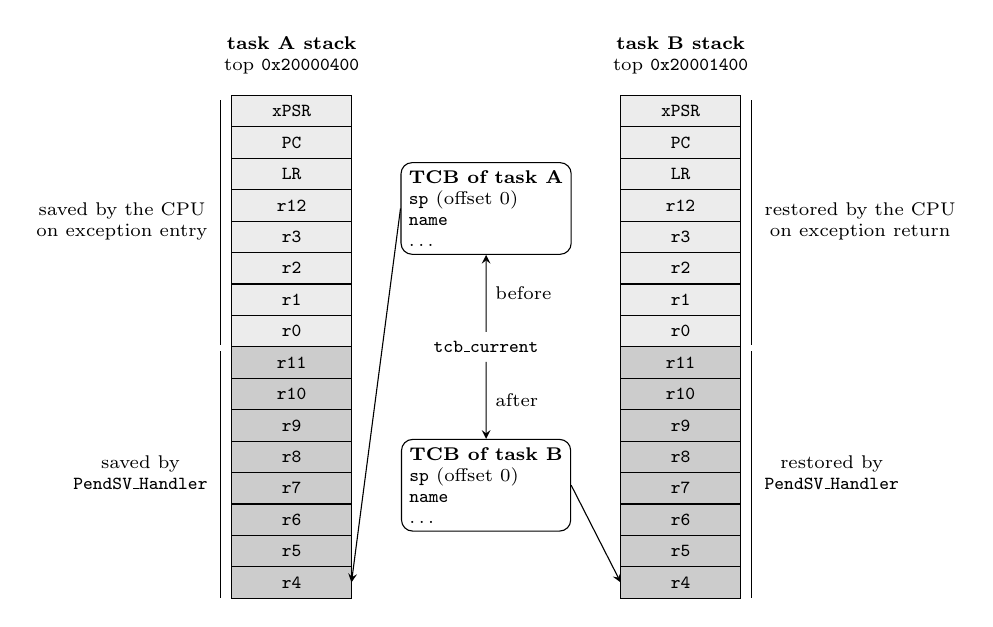
\begin{tikzpicture}[scale=0.95, transform shape,
    reg/.style={draw, minimum width=1.6cm, minimum height=0.42cm, font=\scriptsize\ttfamily, inner sep=0pt},
    tcb/.style={draw, rounded corners, align=left, font=\scriptsize, inner sep=3pt},
    lab/.style={font=\scriptsize, align=center}]
    % task A stack
    \node[lab] at (0,0.75) {\textbf{task A stack}\\top \texttt{0x20000400}};
    \foreach \r [count=\i from 0] in {xPSR,PC,LR,r12,r3,r2,r1,r0}
        \node[reg, fill=gray!15] at (0,{-\i*0.42}) {\r};
    \foreach \r [count=\i from 8] in {r11,r10,r9,r8,r7,r6,r5,r4}
        \node[reg, fill=gray!40] at (0,{-\i*0.42}) {\r};
    % task B stack
    \node[lab] at (5.2,0.75) {\textbf{task B stack}\\top \texttt{0x20001400}};
    \foreach \r [count=\i from 0] in {xPSR,PC,LR,r12,r3,r2,r1,r0}
        \node[reg, fill=gray!15] at (5.2,{-\i*0.42}) {\r};
    \foreach \r [count=\i from 8] in {r11,r10,r9,r8,r7,r6,r5,r4}
        \node[reg, fill=gray!40] at (5.2,{-\i*0.42}) {\r};
    % labels A
    \draw (-0.95,0.15) -- (-0.95,-3.13);
    \node[lab, left] at (-1,-1.47) {saved by the CPU\\on exception entry};
    \draw (-0.95,-3.21) -- (-0.95,-6.51);
    \node[lab, left] at (-1,-4.83) {saved by\\\texttt{PendSV\_Handler}};
    % labels B
    \draw (6.15,0.15) -- (6.15,-3.13);
    \node[lab, right] at (6.2,-1.47) {restored by the CPU\\on exception return};
    \draw (6.15,-3.21) -- (6.15,-6.51);
    \node[lab, right] at (6.2,-4.83) {restored by\\\texttt{PendSV\_Handler}};
    % TCBs
    \node[tcb] (tcbA) at (2.6,-1.3) {\textbf{TCB of task A}\\\texttt{sp} (offset 0)\\\texttt{name}\\\ldots};
    \node[tcb] (tcbB) at (2.6,-5.0) {\textbf{TCB of task B}\\\texttt{sp} (offset 0)\\\texttt{name}\\\ldots};
    \node[font=\scriptsize\ttfamily] (cur) at (2.6,-3.15) {tcb\_current};
    \draw[->, >=stealth] (cur) -- node[right, font=\scriptsize] {before} (tcbA);
    \draw[->, >=stealth] (cur) -- node[right, font=\scriptsize] {after} (tcbB);
    \draw[->, >=stealth] (tcbA.west) -- (0.8,-6.3);
    \draw[->, >=stealth] (tcbB.east) -- (4.4,-6.3);
\end{tikzpicture}
\caption{A switch from A to B. Each TCB's \texttt{sp} points at the lowest saved word (\texttt{r4}) of its task's stack. \texttt{tcb\_current} points at the TCB of the task that runs: the switch saves A, moves \texttt{tcb\_current} to B, and restores B. At the end, PSP points at B's hardware frame.}
\end{figure}

\paragraph{Compared with week 4.} Very similar, with more to save and restore: last week only ``launched'' tasks (one ran, then the other, and the decision was always ``the next task''), so registers were never restored and \texttt{r4}--\texttt{r11} never saved. Now every switch \emph{saves and restores}, a real scheduler decides, and switches happen at \emph{several moments} (tick, yield, delay, exit), which needs a smart solution so that the switch code is not copied or called in many places: PendSV.

\subsection{Inspect: \texttt{struct tcb} in \texttt{kernel/task.h}}
Week 4's \texttt{struct task} became the \textbf{task control block}, \texttt{struct tcb}, renamed for consistency with other OSs (task or process control block, TCB or PCB); \texttt{struct tcb}, \texttt{tcb\_current} and \texttt{tick\_count} follow common RTOS naming.
\begin{lstlisting}[language=C]
struct tcb {
    uint32_t *sp;               /* saved stack pointer, while the task is not running */
    const char *name;           /* short name for messages, e.g. "A" */
    void ( *entry )( void );    /* the function the task runs */
    uint32_t *stack_top;        /* first address above the task's stack */
    uint32_t part_start;        /* lowest address of the partition */
    uint32_t part_end;          /* first address after the partition */
    uint32_t *data_start;       /* the task's variables in RAM: start... */
    uint32_t *data_end;         /* ...and end (exclusive) */
    const uint32_t *data_load;  /* their initial values, stored in FLASH */
    enum task_state state;      /* READY, RUNNING, BLOCKED or FINISHED */
    uint32_t wake_tick;         /* if BLOCKED: the tick at which it is READY again */
};
\end{lstlisting}
New since week 4: \texttt{sp}, \texttt{state} (an \texttt{enum task\_state} value, in \texttt{kernel/task.h}: \texttt{TASK\_READY}, \texttt{TASK\_RUNNING}, \texttt{TASK\_BLOCKED}, \texttt{TASK\_FINISHED}) and \texttt{wake\_tick}. The rest is week 4's: name, entry function, stack top and partition limits (all from the linker script), and the location of the task's variables and of their initial values.

\paragraph{Why must \texttt{sp} be the first field?} Assembly knows nothing of C structs: with \texttt{sp} at offset 0, its address is the TCB's own, so with \texttt{r2 = tcb\_current} a plain \texttt{ldr r0, [r2]} reads it and \texttt{str r0, [r2]} writes it. With \texttt{name} first, the switch would take the name pointer for the stack pointer, load a FLASH address (where the string \texttt{"B"} is stored) as B's stack and crash, while the C side would compile without any warning: hence the comment in \texttt{kernel/task.h}, \texttt{sp} ``MUST stay the first field''.

\paragraph{The task table.} \texttt{tasks[]} (\texttt{kernel/task.c}) holds three TCBs, always in this order: A, B and the \textbf{idle task}. \texttt{NUM\_TASKS} (\texttt{kernel/task.h}) is 3; in \texttt{kernel/task.c}, \texttt{NUM\_APP\_TASKS} is \texttt{NUM\_TASKS - 1}, the \textbf{application} tasks A and B, and \texttt{IDLE\_TCB} is \texttt{\&tasks[NUM\_TASKS - 1]}, the last entry. The table is no longer \texttt{const} as in week 4: \texttt{sp}, \texttt{state} and \texttt{wake\_tick} change at run time.

\subsection{Who does the switch? PendSV}
An \textbf{exception} does the switch: the kind of solution computer architects come up with, which ``normal'' people find completely crazy. Every switch starts with an exception (SysTick, a system call, \dots); the naive approach appends the switch code to every handler that may need it, so the same code sits in several places (tick and system calls), which a programmer should avoid. Instead, such a handler raises another, \textbf{pendable} exception, which runs only after the current one has been served: the two handlers are \textbf{chained}, every handler stays clean, and the switch is written once, in the handler of \textbf{PendSV} (``pendable service call''), a system exception like SVCall and SysTick. Examples: for \textbf{round robin at the tick} (or every few ticks), the SysTick handler, after its many duties, would return to the user program, but since it pended PendSV the CPU goes to the PendSV handler, which switches and returns to the new task; \textbf{a system call that needs a switch}, e.g.\ \texttt{exit} (the scheduler must run when a program ends), is an SVC whose handler pends PendSV, which runs when the SVC handler finishes, and the CPU then returns to the next task.

\paragraph{How to pend PendSV.} Write 1 to bit \texttt{PENDSVSET} (bit 28) of the \textbf{ICSR} (Interrupt Control and State Register, \texttt{0xE000ED04}), as \texttt{task\_request\_switch} in \texttt{kernel/task.c} does with \texttt{SCB->ICSR = SCB\_ICSR\_PENDSVSET;}. Writing 0 to the other bits does nothing, so a plain store is enough (no read-modify-write). Every place that needs a switch only \emph{asks} for it (``another exception is chained after me''), and one handler \emph{does} it; two requests together (a tick and a yield) cost one switch, since the pending bit is set once.

\paragraph{Priorities and tail-chaining.} A pending exception starts only if it is more urgent than the running code (week 3: a lower number is more urgent). \texttt{Reset\_Handler} (\texttt{boot/startup.s}) sets the faults to \texttt{0x00}, SVCall to \texttt{0x80}, SysTick and PendSV to \texttt{0xE0}, the least urgent value this kernel uses; the UART interrupt is at \texttt{0xC0}. So PendSV preempts \emph{no} handler (SysTick is equal, the others more urgent): it runs only when no handler runs, just before the CPU would return to the task. When a handler ends with another exception pending, the CPU goes straight to the next handler without returning to the task: \textbf{tail-chaining}. A PendSV pended in \texttt{SysTick\_Handler} thus runs right after it, never inside it; equal priority also means that SysTick cannot preempt PendSV, so a tick never cuts a switch in half. PendSV therefore always interrupts a \emph{task}: PSP is the running task's stack, and the exception return goes back to thread mode, where the next task must start. Switching inside SysTick would be unsafe too: in most systems the tick is more urgent than some device handlers, and a switch while it interrupts one of them would make that handler return into the wrong task.

\begin{figure}[h]
    \centering
    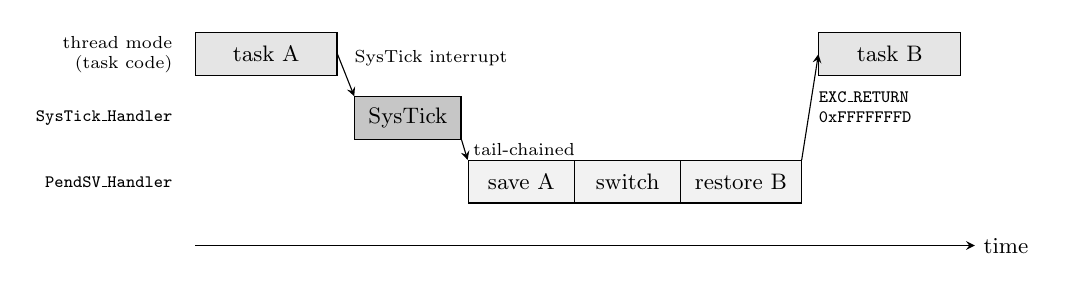
\begin{tikzpicture}[scale=0.9, transform shape, font=\small, >=stealth,
        box/.style={draw, minimum height=0.6cm, inner sep=3pt}]
        \node[left, align=right, font=\scriptsize] at (-0.2,1.8) {thread mode\\(task code)};
        \node[left, font=\scriptsize] at (-0.2,0.9) {\texttt{SysTick\_Handler}};
        \node[left, font=\scriptsize] at (-0.2,0) {\texttt{PendSV\_Handler}};
        % tasks
        \node[box, fill=gray!20, minimum width=2cm] (A) at (1.0,1.8) {task A};
        \node[box, fill=gray!20, minimum width=2cm] (B) at (9.8,1.8) {task B};
        % SysTick
        \node[box, fill=gray!45, minimum width=1.5cm] (S) at (3.0,0.9) {SysTick};
        % PendSV parts
        \node[box, fill=gray!10, minimum width=1.5cm] (P1) at (4.6,0) {save A};
        \node[box, fill=gray!10, minimum width=1.5cm] (P2) at (6.1,0) {switch};
        \node[box, fill=gray!10, minimum width=1.7cm] (P3) at (7.7,0) {restore B};
        % arrows
        \draw[->] (A.east) -- node[above right, font=\scriptsize] {SysTick interrupt} (S.north west);
        \draw[->] (S.south east) -- node[right, font=\scriptsize] {tail-chained} (P1.north west);
        \draw[->] (P3.north east) -- node[right, font=\scriptsize, align=left] {\texttt{EXC\_RETURN}\\\texttt{0xFFFFFFFD}} (B.west);
        \draw[->] (0,-0.9) -- (11,-0.9) node[right] {time};
    \end{tikzpicture}
    \caption{The tick, the request, the switch.}
\end{figure}

\subsection{The switch, step by step: \texttt{PendSV\_Handler} in \texttt{kernel/pendsv.s}}
A and B run unprivileged, on PSP. A runs; at a tick, \texttt{SysTick\_Handler} (\texttt{0xE0}) increments \texttt{tick\_count}, wakes the delayed tasks and decrements \texttt{quantum\_left}, setting \texttt{ICSR.PENDSVSET} when it reaches 0 (the SVCs of \texttt{task\_yield}, \texttt{task\_delay} and \texttt{exit} set it too). Then PendSV does the switch: low-level, so in assembly, but short, 13 instructions (here with their C equivalents).
\begin{lstlisting}
PendSV_Handler:
    mrs   r0, psp            /* sp = PSP: the old task's stack, below its hardware frame */
    stmdb r0!, {r4-r11}      /* sp -= 8; sp[0..7] = r4..r11 */
    ldr   r1, =tcb_current   /* r1 = &tcb_current */
    ldr   r2, [r1]           /* r2 = tcb_current */
    str   r0, [r2]           /* tcb_current->sp = sp (sp is at offset 0) */
    bl    task_switch_context /* task_switch_context(); changes tcb_current */
    ldr   r1, =tcb_current   /* r1 = &tcb_current */
    ldr   r2, [r1]           /* r2 = tcb_current (the new task) */
    ldr   r0, [r2]           /* sp = tcb_current->sp */
    ldmia r0!, {r4-r11}      /* r4..r11 = sp[0..7]; sp += 8 */
    msr   psp, r0            /* PSP = sp: now it points at the hardware frame */
    ldr   r0, =0xFFFFFFFD    /* r0 = EXC_RETURN: thread mode, PSP */
    bx    r0                 /* return_from_exception(0xFFFFFFFD) */
\end{lstlisting}
\begin{enumerate}
    \item \textbf{Entry}: SysTick returns and PendSV is tail-chained. A's hardware frame, pushed on A's stack when SysTick started, is not popped and pushed again: it stays where it is, and only the other registers must be saved.
    \item \textbf{Save A} (the first five instructions). The handler runs on \textbf{MSP}, so \texttt{mrs r0, psp} reads A's stack pointer explicitly. To be fast, \texttt{stmdb r0!, \{r4-r11\}} (``store multiple, decrement before'': registers on the right, destination first) pushes \texttt{r4}--\texttt{r11} with one instruction into the 8 words below \texttt{r0}, \texttt{r4} lowest, and \texttt{!} writes the new, lower address back into \texttt{r0}: a push, but on PSP instead of the handler's own stack. Then \texttt{r0} is stored at offset 0 of \texttt{tcb\_current}, i.e.\ in \texttt{tcb\_current->sp}, as in week 4. The two halves combine: part of the state saved by the hardware on entry, the rest pushed by software, the stack pointer kept in the TCB.
    \item \textbf{Choose}: \texttt{bl task\_switch\_context} calls the C function that marks A READY, picks the next READY task in round-robin order (B), sets \texttt{tcb\_current = B} and programs MPU region 1 for B's partition.
    \item \textbf{Restore B}, the exact opposite: reload \texttt{tcb\_current}, read B's \texttt{sp}, pop \texttt{r4}--\texttt{r11} with \texttt{ldmia} (``load multiple, increment after'', the reverse of \texttt{stmdb}), and \texttt{msr psp, r0} points PSP at what is left: B's hardware frame.
    \item \textbf{Return}: \texttt{0xFFFFFFFD} is the \texttt{EXC\_RETURN} value the link register must hold, on return from an exception, to go back to thread mode (user space) using PSP (week 4). \texttt{bx r0} returns: the hardware pops B's frame, and B continues at the instruction where it was stopped.
\end{enumerate}
PendSV starts in A and ends in B; A notices nothing, since at its next turn steps 4 and 5 give it back exactly the registers it had.

\paragraph{Why may the handler call C without saving \texttt{r0}--\texttt{r3}?} A C function receives its arguments in \texttt{r0}, \texttt{r1}, \texttt{r2}, \dots, returns its result in \texttt{r0}, and may change \texttt{r0}--\texttt{r3}, \texttt{r12} and \texttt{lr}. Nothing of the old task is lost: those registers are in its hardware frame, \texttt{r4}--\texttt{r11} were just pushed (and the C function gives them back unchanged anyway, as the calling rules require), and right after the call all of the new task's registers are restored. And since the handler pushes nothing on MSP, the main stack keeps the \textbf{8-byte alignment} given by the hardware on exception entry, which the C calling rules require when calling a function. \textbf{Warning} (especially for the project): whenever assembly calls C, check very carefully that no register contents are destroyed; the compiler adds instructions to follow the calling convention, and forgetting that they exist leads to strange behaviours.

\paragraph{Why is the entry \texttt{lr} never saved?} On exception entry \texttt{lr} holds an \texttt{EXC\_RETURN} value, not a return address. Every task runs in thread mode on PSP, so the right value is always \texttt{0xFFFFFFFD}, loaded as a constant at the end; the \texttt{lr} received (destroyed by \texttt{bl}) is not needed, and the task's own \texttt{lr} is in its hardware frame, popped by the hardware.

\paragraph{Other remarks.} \texttt{tcb\_current} is read twice, because \texttt{task\_switch\_context()} changes it from the old task to the new one. \texttt{CONTROL} is never touched: \texttt{nPRIV}, set when the first task started (week 4), is never cleared, so every task, B included, runs unprivileged. Interrupts stay enabled: a UART interrupt (\texttt{0xC0}, more urgent) may interrupt PendSV, but never touches PSP or the TCBs; SysTick (same priority) cannot, and SVCall cannot happen while a handler runs.

\subsection{Inspect: \texttt{task\_switch\_context}, the round-robin circle}
Besides step 3 above, it gives the chosen task a fresh slice (\texttt{quantum\_left = QUANTUM}). \texttt{(rr\_last + k) \% NUM\_APP\_TASKS} visits the application tasks in table order, from the one after the last that ran, so A and B alternate: round robin \emph{without a separate queue}, since the table itself is the circle. Not the best possible implementation (it relies on a static array, as there is no dynamic memory), but simple. FINISHED and BLOCKED tasks are never READY, so they are skipped; a preempted task, READY again, goes to the end of the circle. With dynamic memory, a linked list of READY tasks would make round robin even easier (no scan: take the head of the list), but our OS has no \texttt{malloc}.

\paragraph{A's slice ends while B is BLOCKED: who runs?} A is first set READY; the scan starts after \texttt{rr\_last = 0} (A): \texttt{k = 1} tries B (BLOCKED), \texttt{k = 2} A itself (READY), so A runs again with a new slice (Unit 1's ``with no other READY task, the running task keeps the CPU''). Not optimised, though: the tick came, PendSV was chained and A saved before the scheduler finds that A must run again, so A is restored: the \textbf{cost of a switch is paid anyway}, although the running task does not change. Optimisations could avoid it (e.g.\ checking whether a switch is really needed before pending PendSV).

\paragraph{A and B both BLOCKED: who runs?} No task is READY, so \texttt{next} stays \texttt{IDLE\_TCB}: the \textbf{idle task} runs. \texttt{rr\_last} does not change, so afterwards the circle goes on where it stopped.

\subsection{Try it: one switch in gdb}
Run \texttt{make debug} in \texttt{week-05/base} and, in a second terminal in the same folder, \texttt{arm-none-eabi-gdb build/scratch-os.axf}, with breakpoints on the switch code:
\begin{lstlisting}
(gdb) target remote :1234
(gdb) break PendSV_Handler
(gdb) break task_switch_context
(gdb) continue
(gdb) p tick_count
(gdb) p tcb_current->name
(gdb) p/x $psp
(gdb) x/8wx $psp                              # A's hardware frame
(gdb) info symbol *(uint32_t *)($psp + 24)    # the saved pc: word 6
(gdb) info symbol *(uint32_t *)($psp + 20)    # the saved lr: word 5
\end{lstlisting}
\textbf{Rule for gdb this week}: read kernel variables only while the CPU is stopped in a \textbf{handler}, as here. Stopped inside a task (thread mode), the MPU checks gdb's reads too, with the task's rights: \texttt{p tick\_count} fails with \texttt{Cannot access memory}, since \texttt{tick\_count} is in kernel RAM, which an unprivileged task may not read. The output:
\begin{lstlisting}
Breakpoint 1, PendSV_Handler () at kernel/pendsv.s
$1 = 5
$2 = 0x11fc "A"
$3 = 0x200003b8
0x200003b8: 0x00000004 0x00000013 0x00000002 0x00000000
0x200003c8: 0x00000000 0x00001005 0x00001040 0x21000000
task_tick_count + 2 in section .text
spin_ticks + 21 in section .text
\end{lstlisting}
\begin{itemize}
    \item The first switch is at tick 5, the end of A's first slice. The breakpoint is at the first instruction of \texttt{PendSV\_Handler}: nothing is saved yet, and \texttt{tcb\_current} is still A.
    \item PSP $=$ \texttt{0x200003b8}, inside A's stack (\texttt{0x20000000}--\texttt{0x20000400}); the 8 words are the frame pushed on SysTick entry: \texttt{r0}--\texttt{r3}, \texttt{r12}, then \texttt{lr = 0x1005}, \texttt{pc = 0x1040}, \texttt{xPSR = 0x21000000}.
    \item The saved \texttt{pc} is in \texttt{task\_tick\_count}: A was stopped in its busy work, which calls that stub in a loop, and the saved \texttt{lr} returns into \texttt{spin\_ticks}. \texttt{xPSR} has the T bit (\texttt{0x01000000}) and the C flag (\texttt{0x20000000}) of A's last comparison.
    \item With a compiler version other than the course one the addresses may differ slightly; the meaning is the same.
\end{itemize}

\paragraph{Continue: A saved, B chosen.} Same session; \texttt{0xE000ED9C} is the MPU's \texttt{MPU\_RBAR} (week 4), the next word \texttt{MPU\_RASR}.
\begin{lstlisting}
(gdb) continue                    # stops in task_switch_context
(gdb) p tcb_current->sp
(gdb) x/8wx tcb_current->sp       # A's r4..r11
(gdb) x/2wx 0xE000ED9C            # MPU region 1 now
(gdb) finish                      # run to the end of the function
(gdb) p tcb_current->name
(gdb) p tcb_current->sp
(gdb) x/16wx tcb_current->sp      # B's stack
(gdb) x/2wx 0xE000ED9C            # MPU region 1 after the choice
\end{lstlisting}
B has never run: what do you expect in its 16 words? The output:
\begin{lstlisting}
Breakpoint 2, task_switch_context () at kernel/task.c
$4 = (uint32_t *) 0x20000398
0x20000398: 0x00000002 0x00000000 0x00000000 0x200003d8
0x200003a8: 0x00000000 0x00000000 0x00000000 0x00000000
0xe000ed9c: 0x20000001 0x13060017
PendSV_Handler () at kernel/pendsv.s
$5 = 0x1200 "B"
$6 = (uint32_t *) 0x200013c0
0x200013c0: 0x00000000 0x00000000 0x00000000 0x00000000
0x200013d0: 0x00000000 0x00000000 0x00000000 0x00000000
0x200013e0: 0x00000000 0x00000000 0x00000000 0x00000000
0x200013f0: 0x00000000 0x00001043 0x000010c4 0x01000000
0xe000ed9c: 0x20001001 0x13060017
\end{lstlisting}
\begin{itemize}
    \item A's saved \texttt{sp} is \texttt{0x20000398} $=$ \texttt{0x200003b8} $-$ 32: \texttt{stmdb} pushed A's \texttt{r4}--\texttt{r11} (8 registers, 32 bytes) below the hardware frame, with their values at the moment A was stopped.
    \item \texttt{finish} runs to the end of \texttt{task\_switch\_context} and stops back in \texttt{PendSV\_Handler}, just after the \texttt{bl}: \texttt{tcb\_current} is now B.
    \item B's 16 words: 8 zeros for \texttt{r4}--\texttt{r11}, then a hardware frame with \texttt{r0}--\texttt{r3}, \texttt{r12} $= 0$, \texttt{lr = 0x1043} (\texttt{task\_exit}, with the Thumb bit set), \texttt{pc = 0x10c4} (\texttt{task\_b}) and \texttt{xPSR = 0x01000000} (T bit only). B never ran, so nobody ever saved it: it is a \textbf{fake} frame (next subsection).
    \item \texttt{MPU\_RBAR} went from \texttt{0x20000001} (A's partition, region 1) to \texttt{0x20001001} (B's partition, region 1): the choice moved the MPU window.
\end{itemize}
Quit gdb with \texttt{quit} (answer \texttt{y}), and QEMU with \texttt{Ctrl-C} in its terminal.

\subsection{The first run of a task: a fake frame}
In week 4 a task's first run was a \textbf{fake exception}: \texttt{task\_launch} wrote an 8-word hardware frame on its stack and returned into it, as if from an exception. This now proves useful, since every run of a task is assumed to come from an exception, even the very first; but a first run must now look like a \textbf{full context switch}, because PendSV switches to B, which never ran and was never saved, exactly as it switches back to A (load \texttt{sp}, pop 8 words, set PSP, return). So the fake frame must be \emph{bigger}:
\begin{itemize}
    \item At boot, \texttt{task\_init\_stack} builds on \textbf{every} task's stack what PendSV would have left had the task been switched out just before its first instruction: the 8-word hardware frame \textbf{plus} 8 words for \texttt{r4}--\texttt{r11} below it, with \texttt{t->sp} at the lowest word. The first switch to a task is then identical to every later one (PendSV believes the task was running, finds everything correctly in memory, and the task starts): no special case for a new task.
    \item Only the very first task, A, is entered differently: \texttt{main}'s \texttt{svc \#5} (\texttt{SYS\_START\_TASKS}) ends in \texttt{task\_start\_first} (\texttt{kernel/task.c}), which sets PSP to \texttt{sp + 8}, i.e.\ to the hardware frame, skipping the 8 zeros for \texttt{r4}--\texttt{r11} because the exception return pops only the hardware frame; then it sets nPRIV and returns from SVCall with \texttt{0xFFFFFFFD}, as in week 4.
\end{itemize}

\paragraph{Inspect: \texttt{task\_init\_stack} in \texttt{kernel/task.c}.} \texttt{task\_start\_first} calls it once per task (A, B and idle) before the first task starts, together with week 4's \texttt{partition\_init} and with setting the state to READY. The 16 words for task B (stack top \texttt{0x20001400}) are the ones gdb showed:
\begin{center}
    \begin{tabular}{l l l l}
        \hline
        \textbf{Words} & \textbf{Addresses (task B)} & \textbf{Register} & \textbf{Value written} \\
        \hline
        \texttt{regs[0..7]} & \texttt{0x200013c0}--\texttt{0x200013df} & \texttt{r4}\ldots\texttt{r11} & 0 (PendSV pops them) \\
        \texttt{frame[0..4]} & \texttt{0x200013e0}--\texttt{0x200013f3} & \texttt{r0}, \texttt{r1}, \texttt{r2}, \texttt{r3}, \texttt{r12} & 0 \\
        \texttt{frame[5]} & \texttt{0x200013f4} & \texttt{lr} & \texttt{task\_exit} \\
        \texttt{frame[6]} & \texttt{0x200013f8} & \texttt{pc} & \texttt{t->entry \& \textasciitilde 1u}: \texttt{task\_b} \\
        \texttt{frame[7]} & \texttt{0x200013fc} & \texttt{xPSR} & \texttt{0x01000000} (\texttt{XPSR\_THUMB}) \\
        \hline
    \end{tabular}
\end{center}
The heart of the function:
\begin{lstlisting}[language=C]
    uint32_t *frame = t->stack_top - 8;   /* the hardware frame: 8 words below the top */
    ...                                   /* frame[0..7] as in the table */
    uint32_t *regs = frame - 8;           /* 8 more words for r4..r11 */
    for ( int i = 0; i < 8; i++ )
        regs[i] = 0;                      /* r4 + i = 0 */
    t->sp = regs;                         /* the saved stack pointer */
\end{lstlisting}
\begin{itemize}
    \item B's saved \texttt{sp} is \texttt{0x200013c0}: 16 words are 64 bytes (\texttt{0x40}), and \texttt{0x20001400} $-$ \texttt{0x40} $=$ \texttt{0x200013c0}.
    \item \texttt{r4}--\texttt{r11} may start as 0: a C function never reads them before writing them (it only saves and restores them for its caller), so any value works for a task's first instruction.
    \item \texttt{lr}, \texttt{pc} and T bit work as in week 4's \texttt{task\_launch}: the \texttt{pc} is the entry function with bit 0 cleared, since the popped \texttt{pc} must be a real instruction address; \texttt{xPSR} needs the T (Thumb) bit, or the first instruction faults; \texttt{lr} is \texttt{task\_exit} (\texttt{lib/syscalls.s}), which calls \texttt{sys\_exit} when \texttt{task\_b} returns: returning from a task's function means exit.
\end{itemize}

\subsection{One MPU window, moved at every switch}
Already implemented in week 4. On a single core one task runs at a time, so the MPU needs only \textbf{one task region}, which the kernel keeps moving onto the running task: at the end of every scheduling decision, \texttt{task\_switch\_context()} takes the next task's partition limits from its TCB and calls \texttt{mpu\_set\_task\_region()} with the partition's start and size. RAM holds three 4\,KB partitions (A at \texttt{0x20000000}, B at \texttt{0x20001000}, idle at \texttt{0x20002000}), with the kernel's RAM above; region 0 is FLASH, read-only, executable and shared by all.
\begin{figure}[h]
    \centering
    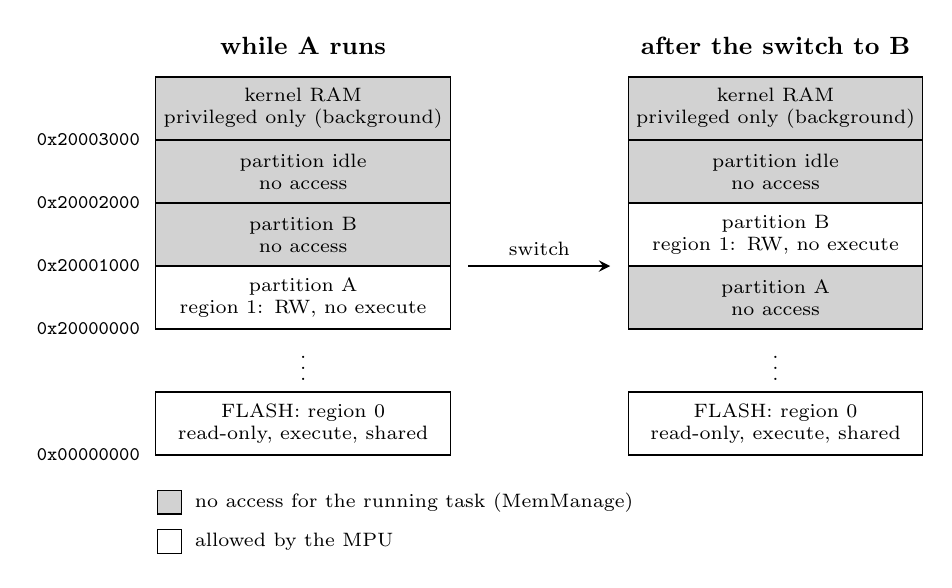
\begin{tikzpicture}[font=\scriptsize,
        mem/.style={draw, text width=3.6cm, minimum height=0.8cm, align=center, inner sep=2pt},
        ok/.style={mem, fill=white},
        no/.style={mem, fill=gray!35}]
        % left: while A runs
        \node[font=\small\bfseries] at (0,4.0) {while A runs};
        \node[no] at (0,3.2) {kernel RAM\\privileged only (background)};
        \node[no] at (0,2.4) {partition idle\\no access};
        \node[no] at (0,1.6) {partition B\\no access};
        \node[ok] at (0,0.8) {partition A\\region 1: RW, no execute};
        \node at (0,0) {$\vdots$};
        \node[ok] at (0,-0.8) {FLASH: region 0\\read-only, execute, shared};
        \foreach \y/\a in {2.8/0x20003000, 2.0/0x20002000, 1.2/0x20001000, 0.4/0x20000000, -1.2/0x00000000}
            \node[left, font=\scriptsize\ttfamily] at (-1.95,\y) {\a};
        % right: after the switch to B
        \node[font=\small\bfseries] at (6,4.0) {after the switch to B};
        \node[no] at (6,3.2) {kernel RAM\\privileged only (background)};
        \node[no] at (6,2.4) {partition idle\\no access};
        \node[ok] at (6,1.6) {partition B\\region 1: RW, no execute};
        \node[no] at (6,0.8) {partition A\\no access};
        \node at (6,0) {$\vdots$};
        \node[ok] at (6,-0.8) {FLASH: region 0\\read-only, execute, shared};
        % arrow
        \draw[->, >=stealth, thick] (2.1,1.2) -- node[above] {switch} (3.9,1.2);
        % legend
        \node[draw, fill=gray!35, minimum size=0.3cm] at (-1.7,-1.8) {};
        \node[right] at (-1.5,-1.8) {no access for the running task (MemManage)};
        \node[draw, fill=white, minimum size=0.3cm] at (-1.7,-2.3) {};
        \node[right] at (-1.5,-2.3) {allowed by the MPU};
    \end{tikzpicture}
    \caption{\texttt{task\_switch\_context()} calls \texttt{mpu\_set\_task\_region()} for the new task: \texttt{MPU\_RBAR} goes from \texttt{0x20000001} to \texttt{0x20001001}.}
\end{figure}

\paragraph{Try it: a rogue task after a switch.} Does week 4's isolation survive the switches? With \texttt{DEMO=rogue}, B stores \texttt{0x12345678} into the kernel's \texttt{uptime\_ms}, as in week 4, but only after A's first slice, i.e.\ \textbf{after a context switch}.
\begin{lstlisting}[language=bash]
    make DEMO=rogue run
\end{lstlisting}
The demo builds into \texttt{build/demo-rogue/}. Output (quit QEMU with \texttt{Ctrl-C}):
\begin{verbatim}
    scratch-os: kernel started
    scheduler: round robin, quantum 5 ticks
    A: hello from task A
    A: step 1 (tick 2)
    A: step 2 (tick 4)
    B: hello from task B
    B: writing to the kernel's uptime counter
    MemManage: CFSR=0x82
    address 0x20003094
    cause: data access
\end{verbatim}
\begin{itemize}
    \item \texttt{0x20003094} is \texttt{uptime\_ms} (\texttt{drivers/systick.c}), in kernel RAM above the three partitions (a little higher in the solution, whose trace buffer also lives in kernel RAM). \texttt{CFSR = 0x82}: as in week 4, a data access violation (\texttt{DACCVIOL}) with a valid fault address (\texttt{MMARVALID}).
    \item \textbf{Which MPU region decides on B's store?} Region 1, set by the switch at tick 5 to B's partition, \texttt{0x20001000}--\texttt{0x20002000}. Kernel RAM is reachable only through the privileged background region, and B is unprivileged: the store faults, \textbf{exactly as in week 4}. A's partition is off limits to B too: after the switch, no region describes it for B. \texttt{MemManage\_Handler} (\texttt{kernel/faults.c}) then stops the whole system, as in week 4.
\end{itemize}

\subsection{SysTick, the time slice and \texttt{task\_increment\_tick}}
The \textbf{system tick} is the hardware interrupt, every \textbf{10\,ms} here (week 3's SysTick); the \textbf{time slice} is round robin's quantum, implemented by \textbf{counting ticks}. The scheduler gets control only at a tick, so the quantum must be a \textbf{multiple of the tick}: one that is not (e.g.\ shorter than a tick) is meaningless, as the task is interrupted only every 10\,ms anyway. The tick period is set by programming the hardware counter, so tick and scheduler must be designed together. Since this week, \texttt{SysTick\_Handler} (\texttt{drivers/systick.c}) also calls \texttt{task\_increment\_tick()}, which drives the scheduler; like all kernel functions from now on, it works by updating the TCBs.
\begin{lstlisting}[language=C]
void task_increment_tick( void )
{
    tick_count++;
    if ( tcb_current == 0 ) return;                 /* no task started yet */

    int woke = 0;
    for ( unsigned i = 0; i < NUM_APP_TASKS; i++ )
        if ( tasks[i].state == TASK_BLOCKED
             && ( int32_t ) ( tick_count - tasks[i].wake_tick ) >= 0 )
        {
            tasks[i].state = TASK_READY; woke = 1;  /* may run again */
        }

    if ( tcb_current == IDLE_TCB )                  /* idle: leave it only if a task woke */
    {
        if ( woke ) task_request_switch();
        return;
    }

#if QUANTUM > 0
    quantum_left--;
    if ( quantum_left == 0 ) task_request_switch(); /* SCB->ICSR = PENDSVSET */
#endif
}
\end{lstlisting}
At every tick:
\begin{itemize}
    \item \textbf{\texttt{tick\_count++}}: the kernel's clock, in ticks since the scheduler started, read by tasks with the system call \texttt{task\_tick\_count()}. \texttt{tcb\_current} is 0 until the first task starts (\texttt{main} starts SysTick before the tasks), and until then the function only counts.
    \item \textbf{Wake up}: the tick is usually where the kernel wakes blocked tasks. The delay (sleep) system call, modified, now sets the task BLOCKED (here delays are the only way to block, the task saying how many ticks it sleeps); at each tick, every BLOCKED application task whose \texttt{wake\_tick} has come becomes READY (BLOCKED $\to$ READY). A task that sleeps 10\,ms (one tick) is detected by the loop at the following tick.
    \item \textbf{The time slice}: the kernel does not schedule at every tick; with a 10\,ms tick and a 100\,ms quantum, it counts the ticks since the start of the current quantum and schedules only when it is over. \texttt{quantum\_left}, the ticks left to the running task, starts at \texttt{QUANTUM} (5 by default, a \texttt{\#define} in \texttt{kernel/task.h} that the Makefile can change); at 0, \texttt{task\_request\_switch()} pends PendSV, which runs the scheduler.
    \item \textbf{\texttt{QUANTUM = 0}} means ``never switch on the tick'': \texttt{\#if QUANTUM > 0} removes the slice code completely, and tasks keep the CPU until they block, yield or exit, passing control to each other: Unit 1's \textbf{cooperative} scheduling.
\end{itemize}
A woken task does nothing at once: READY, it waits for the end of the running task's slice (Unit 1's rules); only the idle task gives way at once, because when \texttt{woke} is set during idle the tick asks for a switch immediately. Nor is the quantum \textbf{aligned to a global grid} (from a question in class): if a task stops after 1\,ms of a 100\,ms quantum (it blocks, yields or exits), the next task does not wait for a ``quantum boundary'': it runs as soon as the CPU is free, with its quantum starting then (\texttt{quantum\_left = QUANTUM} in \texttt{task\_switch\_context}).

\paragraph{Why \texttt{(int32\_t)(tick\_count - wake\_tick) >= 0} and not \texttt{tick\_count >= wake\_tick}?} After $2^{32}$ ticks (about 497 days at 10\,ms) \texttt{tick\_count} wraps around to 0, and a plain comparison fails: a wake-up tick just before the wrap would look far in the future. The unsigned difference read as signed stays correct across the wrap (for values less than $2^{31}$ ticks apart), like week 3's \texttt{now - start} test.

\paragraph{Lesson: an OS is many small parts working together.} The code is simpler than it looks on slides: many small, very simple parts working together, and building an OS means spending a lot of time checking that they are linked properly: e.g.\ \texttt{task\_request\_switch} is called from the system-call exceptions but also from \texttt{task\_increment\_tick}, and every event that can happen must be kept under control. Every single bug can crash the system. Big bugs are not really a problem: the system crashes and they get fixed. The nightmare is small hidden bugs that show up only in rare corner cases: everything seems fine, then suddenly the OS crashes.

\subsection{Try it: change the quantum}
The quantum is a Makefile variable, easy to experiment with. With 2 ticks:
\begin{lstlisting}[language=bash]
    make QUANTUM=2 run
\end{lstlisting}
The build goes into its own folder, \texttt{build/quantum-2/}, never mixing with the default one. Output (quit QEMU with \texttt{Ctrl-C}):
\begin{verbatim}
    scratch-os: kernel started          A: step 7 (tick 28)
    scheduler: round robin, quantum 2   B: step 7 (tick 30)
    A: hello from task A                A: step 8 (tick 32)
    B: hello from task B                B: step 8 (tick 34)
    A: step 1 (tick 4)                  A: step 9 (tick 36)
    B: step 1 (tick 6)                  B: step 9 (tick 38)
    A: step 2 (tick 8)                  A: step 10 (tick 40)
    B: step 2 (tick 10)                 task A exited (tick 40)
    A: step 3 (tick 12)                 B: step 10 (tick 40)
    B: step 3 (tick 14)                 B: step 11 (tick 42)
    A: step 4 (tick 16)                 B: step 12 (tick 44)
    B: step 4 (tick 18)                 B: step 13 (tick 46)
    A: step 5 (tick 20)                 B: step 14 (tick 48)
    B: step 5 (tick 22)                 B: step 15 (tick 50)
    A: step 6 (tick 24)                 task B exited (tick 50)
    B: step 6 (tick 26)                 all tasks finished
\end{verbatim}
Compared with the default quantum of 5:
\begin{itemize}
    \item \textbf{One step per turn}: a 2-tick slice is one step. A's slice ends at tick 2, just as step 1 would end; back on the CPU at 4, the step is over and A prints it. So each line is printed at the \emph{start} of a turn of its task.
    \item \textbf{A finishes at tick 40 (not 32), B at 50 (not 44)}: the busy work counts clock ticks, also while the task is switched out, and a step ending with its slice is printed only at the task's next turn, 2 ticks later, so while both tasks run every step costs 4 ticks of clock time.
    \item \textbf{21 switches instead of 7} (counted by the trace): Unit 1's overhead $s/(q+s)$ grows as $q$ shrinks.
\end{itemize}

\subsection{Task states in the code}
Unit 1's states are \texttt{enum task\_state} (\texttt{kernel/task.h}), and each transition is one line of \texttt{kernel/task.c}:
\begin{center}
    \begin{tabular}{l l l}
        \hline
        \textbf{Transition} & \textbf{When} & \textbf{Where in the code} \\
        \hline
        $\to$ READY & at boot, for every task & \texttt{task\_start\_first} \\
        READY $\to$ RUNNING & the task is chosen & \texttt{task\_switch\_context} \\
        RUNNING $\to$ READY & preempted or yield & \texttt{task\_switch\_context} \\
        RUNNING $\to$ BLOCKED & delay, delay until & \texttt{task\_block\_until} \\
        BLOCKED $\to$ READY & its \texttt{wake\_tick} has come & \texttt{task\_increment\_tick} \\
        RUNNING $\to$ FINISHED & the task calls exit (or returns) & \texttt{task\_finish\_current} \\
        \hline
    \end{tabular}
\end{center}
READY $\to$ RUNNING and RUNNING $\to$ READY are both in \texttt{task\_switch\_context}, since with round robin a switch removes one task from the CPU and starts another. There is no BLOCKED $\to$ RUNNING (a woken task waits as READY), and exactly one task is RUNNING (\texttt{tcb\_current}): the idle task, if no other can.

\subsection{Giving the CPU away: yield, delay, delay until, exit}
Three new system calls (declared in \texttt{lib/syscalls.h}) leave the CPU before the slice ends: each is an \texttt{svc} whose service (\texttt{kernel/syscall.c}) pends PendSV, which, less urgent (\texttt{0xE0}) than SVCall (\texttt{0x80}), waits and runs right after the \texttt{svc}, tail-chained.
\begin{itemize}
    \item \textbf{\texttt{task\_yield()}} (\texttt{svc \#6}, \texttt{sys\_yield\_impl}): ``let the other task run now''; the task stays READY and goes to the end of the circle, and the scheduler picks it again if no other task is READY.
    \item \textbf{\texttt{task\_delay(ticks)}} (\texttt{svc \#7}, \texttt{sys\_delay\_impl}): BLOCKED until \texttt{tick\_count} reaches now $+$ \texttt{ticks}.
    \item \textbf{\texttt{task\_delay\_until(\&last, period)}} (\texttt{svc \#8}, \texttt{sys\_delay\_until\_impl}): BLOCKED until tick \texttt{last + period}, with \texttt{last} moved to that tick.
\end{itemize}

\paragraph{Why two delays?} \texttt{task\_delay} waits a number of ticks counted from the call, ignoring the time the task already spent (on its work, in the system call, waiting for the CPU): inconvenient for a \textbf{periodic task}. A task that must run every 2 seconds is an infinite loop of ``some activity, then wait''; with \texttt{delay} it would have to compute how long its activity took and delay only for the rest, which is very difficult, and a loop ``work, then \texttt{delay(10)}'' has a period of work $+$ 10 ticks $+$ any wait for the CPU: it \textbf{drifts}, and is never exact. With \texttt{task\_delay\_until} the task tells the OS ``this was the beginning of my periodic activation, and I want one every 2 seconds'': if the work took 1 second, the OS makes it wait just 1 more. Wake-ups stay at \texttt{last + period}, \texttt{last + 2$\cdot$period}, \dots\ however long the work took (as long as it is shorter than the period): \textbf{no drift}; \texttt{last} is set once, with \texttt{task\_tick\_count()}, before the loop. For the scheduler both calls just block the task, but they are implemented differently, and a periodic task (one that must run every $T$ ticks) needs \texttt{task\_delay\_until}. Both exist in FreeRTOS, where programming is largely about using them: this is why they were implemented here.

\paragraph{Exit.} \texttt{sys\_exit\_impl} calls \texttt{task\_finish\_current}, which marks the task FINISHED (RUNNING $\to$ FINISHED) and pends PendSV; the task is never chosen again. When only the idle task is left, \texttt{task\_finish\_current} prints \texttt{all tasks finished}; QEMU keeps running after that line because the idle task runs forever. Unlike week 4, \texttt{main} never gets the CPU back.

\paragraph{Inspect: \texttt{task\_block\_until} and the delay services.} The two delay services share one helper, \texttt{task\_block\_until} (\texttt{kernel/task.c}):
\begin{lstlisting}[language=C]
void task_block_until( uint32_t wake_tick )
{
    tcb_current->wake_tick = wake_tick;         /* when to wake up */
    tcb_current->state = TASK_BLOCKED;          /* not READY until then */
    task_request_switch();                      /* give the CPU to another task */
}
\end{lstlisting}
The body of \texttt{sys\_delay\_impl} (\texttt{kernel/syscall.c}; \texttt{a0} is the number of ticks):
\begin{lstlisting}[language=C]
    if ( a0 == 0 )
        task_request_switch();                  /* delay(0) = yield */
    else
        task_block_until( tick_count + a0 );    /* READY again at tick now + a0 */
\end{lstlisting}
and of \texttt{sys\_delay\_until\_impl} (\texttt{a0} is the address of \texttt{last\_wake}, \texttt{a1} the period, \texttt{t} is \texttt{tcb\_current}):
\begin{lstlisting}[language=C]
    if ( !in_range( a0, sizeof( uint32_t ), t->part_start, t->part_end )
         || ( a0 & 3 ) != 0 )
        return ( uint32_t ) -1;
    uint32_t *last_wake = ( uint32_t * ) a0;    /* the number is really an address */
    uint32_t wake = *last_wake + a1;            /* the next wake-up tick */
    *last_wake = wake;                          /* remembered for the next period */
    if ( ( int32_t ) ( wake - tick_count ) > 0 )
        task_block_until( wake );
\end{lstlisting}
Both services first return $-1$ if no task has started yet.
\begin{itemize}
    \item \textbf{Why the \texttt{in\_range} check?} The kernel \textbf{writes} \texttt{*last\_wake}, and it runs privileged, so the MPU would not stop it: without the check, a task could pass the address of a kernel variable and have the kernel overwrite it (the lesson of week 4's \texttt{sys\_write} check). Only an address inside the caller's own partition, aligned to 4 like every \texttt{uint32\_t}, is accepted.
    \item \textbf{What if the task calls \texttt{task\_delay\_until} after its wake-up tick?} If \texttt{wake} is not in the future, the test is false: the task does \textbf{not} block, but continues at once, to catch up. \texttt{last} still moves by one period, so the later wake-ups stay on the same grid.
    \item \textbf{Where does the task go on afterwards?} PendSV switched away right after the \texttt{svc}, saving the \texttt{pc} that follows it: when chosen again, the task resumes there, returns into the stub (\texttt{task\_delay} in \texttt{lib/syscalls.s}), and the stub returns to the caller.
\end{itemize}

\subsection{Try it: no preemption, no yield}
In a cooperative system, a task that never gives the CPU away freezes the others (Unit 1). \texttt{DEMO=coop} shows it: \texttt{QUANTUM} is 0, so the tick never switches (the \texttt{Makefile} forces it with \texttt{override}), and task A loops forever on its busy work, never yielding.
\begin{lstlisting}[language=bash]
    make DEMO=coop run
\end{lstlisting}
Let it run for a few seconds, then quit QEMU with \texttt{Ctrl-C}:
\begin{verbatim}
    scratch-os: kernel started
    scheduler: round robin, quantum 0 ticks
    A: hello from task A
    A: step 1 (tick 0)
    A: step 2 (tick 2)
    A: step 3 (tick 4)
    ...
    A: step 182 (tick 362)
\end{verbatim}
\begin{itemize}
    \item \textbf{Task B never prints anything}, while A's step number grows as long as QEMU runs: B is READY all the time, but nobody takes the CPU from A, and A never gives it away. B \textbf{starves}.
    \item \textbf{The fix is a yield}: \texttt{task\_yield();} at the end of A's loop body (\texttt{src/task\_a.c}) makes A give the CPU away after each step. B then runs, but its own loop never yields, so now \textbf{A} waits until B has finished its 15 steps; with \texttt{task\_yield();} in the loops of \textbf{both} tasks, they alternate one step each, as with a quantum of 2. In a cooperative system every task must play fair: one loop without a yield or a delay freezes all the others.
\end{itemize}

\subsection{The idle task}
When A and B are both BLOCKED (or FINISHED), the CPU runs the idle task, the last entry of \texttt{tasks[]}: Unit 1's question answered. It does nothing, and runs whenever there is nothing else to do: where week 4's task B ended with an infinite loop, now A and B both end, and then the idle task runs forever, as in real operating systems.
\begin{itemize}
    \item It is a task like the others: unprivileged, with its own stack and its own 4\,KB partition (\texttt{0x20002000}--\texttt{0x20003000}, placed by the linker script by its file name, \texttt{idle.o}), so the switch, the MPU and the stacks need no special case for it.
    \item It is never in the round-robin circle (\texttt{task\_switch\_context} picks it only when no application task is READY), and it has no time slice: with no task able to run, switching makes no sense, so \texttt{task\_increment\_tick} leaves it only when a task wakes up.
    \item \textbf{Why not a loop inside the kernel?} Kernel code runs in handlers, and a looping handler blocks every exception of the same or lower urgency: PendSV and SysTick (\texttt{0xE0}) could never run, so no tick would come, no task would wake, and no switch would happen.
    \item It waits with \texttt{wfi} (``wait for interrupt'', allowed in unprivileged code): the core stops executing until the next interrupt, which saves energy.
\end{itemize}
The whole task is \texttt{idle\_task} in \texttt{src/idle.c}:
\begin{lstlisting}[language=C]
void idle_task( void )
{
    for ( ;; )
    {
        __asm volatile ( "wfi" );       /* sleep until the next interrupt */
    }
}
\end{lstlisting}
At the latest the next SysTick, 10\,ms away, wakes the CPU from \texttt{wfi}: \texttt{task\_increment\_tick} runs, and if a delayed task is READY again it pends PendSV, so the exception return goes into that task instead of the idle task. Otherwise the handler returns into the idle task right after its \texttt{wfi}, and the loop sends it back to sleep until the next tick. The idle task never returns: an \texttt{exit} from it would leave the CPU with nothing to run.

\paragraph{Try it: delays and the idle task.} With \texttt{make DEMO=idle run}, both tasks do 5 steps of 1 tick of work each: A prints, works 1 tick and calls \texttt{task\_delay(10)}; B calls \texttt{task\_delay\_until(\&last, 6)}, then prints and works 1 tick, with \texttt{last} starting at B's first tick. Output, in chronological order:
\begin{verbatim}
    scratch-os: kernel started
    scheduler: round robin, quantum 5 ticks
    A: hello from task A
    A: step 1 (tick 0)
    B: hello from task B
    B: step 1 (tick 7)
    A: step 2 (tick 11)
    B: step 2 (tick 13)
    B: step 3 (tick 19)
    A: step 3 (tick 22)
    B: step 4 (tick 25)
    B: step 5 (tick 31)
    task B exited (tick 32)
    A: step 4 (tick 33)
    A: step 5 (tick 44)
    task A exited (tick 55)
    all tasks finished
\end{verbatim}
\begin{itemize}
    \item A drifts: steps at 0, 11, 22, 33, 44, a period of 11 $=$ 1 tick of work $+$ 10 of delay; it exits at 55, after its last delay.
    \item B does not: \texttt{last} starts at 1, and B wakes at 7, 13, 19, 25, 31, exactly every 6 ticks, despite its 1 tick of work.
    \item Most of the time both tasks are BLOCKED and the idle task runs, until the tick at which a task wakes up.
\end{itemize}

\subsection{Seeing the schedule: a trace}
The output shows when each step \emph{ended}, not who had the CPU at each tick. To check that many tasks run correctly, and to draw Unit 1's Gantt chart of a real run, the kernel must log its execution, \textbf{writing down every switch}. Logging inside an OS is hard: \texttt{printf} cannot simply be added anywhere, and where it can it is very slow, so in the scheduler, which must be fast, it would completely destroy the timing of the tasks. The trace is therefore ``smart'': events are logged in memory and printed later, when there is time. \texttt{week-05/solution/} has it; the next subsections write it in \texttt{week-05/base/}, at its \texttt{CLASS} comments. The design:
\begin{itemize}
    \item \textbf{One record per switch}: the tick and the indexes in \texttt{tasks[]} of the task that stopped (\texttt{from}) and of the one that starts (\texttt{to}). Between two records the \texttt{to} of the first one owned the CPU, so the records are enough to rebuild the whole chart.
    \item \textbf{Recorded in \texttt{task\_switch\_context}}, the one place every switch passes through, and only when the task really changes (``A keeps the CPU'' is not a switch).
    \item \textbf{Kept in RAM, printed later}: printing inside PendSV would slow every switch and change the very schedule we want to observe, while writing 8 bytes is fast.
    \item \textbf{A ring buffer} of 64 records: when full, the next record overwrites the \textbf{oldest}. A counter \texttt{count} of all the records ever written gives the next slot, \texttt{count \% 64}, and tells how many are still stored.
    \item \textbf{Printed by a system call}: just before returning, task B calls \texttt{trace\_dump()} (\texttt{svc \#9}, already prepared: its service \texttt{sys\_trace\_dump\_impl} in \texttt{kernel/syscall.c} calls \texttt{trace\_print}). \texttt{trace\_print} prints \texttt{TRACE BEGIN}, one line \texttt{T <tick> <from> <to>} per record (oldest first), \texttt{TRACE END <tick now>}, then a small Gantt chart; the course tool \texttt{schedsim} reads the same lines.
    \item The interface is prepared in \texttt{kernel/trace.h}: \texttt{trace\_record\_switch( uint8\_t from, uint8\_t to )} and \texttt{trace\_print( void )}. You write \texttt{kernel/trace.c} at its \texttt{CLASS} comments, plus one call in \texttt{kernel/task.c}.
\end{itemize}
No lock protects the buffer, and none is needed: \texttt{trace\_record\_switch} runs inside PendSV and \texttt{trace\_print} inside SVCall, which never interrupt each other in the middle of their work (PendSV runs only when SVCall is over).

\subsection{Writing the trace: record, buffer and recording}
In \texttt{week-05/base/kernel/trace.c}, the comment \texttt{/* CLASS: trace record type goes here */} becomes the record type:
\begin{lstlisting}[language=C]
/* One task switch. */
struct trace_record {
    uint32_t tick;      /* the tick at which the switch happened */
    uint8_t from;       /* index in the task table of the task that stopped */
    uint8_t to;         /* index in the task table of the task that starts */
};
\end{lstlisting}
and \texttt{/* CLASS: ring buffer goes here */} the buffer:
\begin{lstlisting}[language=C]
/* How many records the buffer holds. */
#define TRACE_SIZE 64

/* The buffer is a ring: when it is full, a new record overwrites the oldest one. */
static struct trace_record buffer[TRACE_SIZE];
/* How many records were written in all. The next one goes to slot count % TRACE_SIZE. */
static uint32_t count = 0;
\end{lstlisting}
\texttt{buffer} and \texttt{count} are \texttt{static}, visible only in \texttt{kernel/trace.c}: kernel variables, in kernel RAM, which no task can read or change. Inside \texttt{trace\_record\_switch}, the three placeholder lines (\texttt{(void) from;}, \texttt{(void) to;} and the \texttt{CLASS} comment) become:
\begin{lstlisting}[language=C]
    struct trace_record *r = &buffer[count % TRACE_SIZE];   /* the next slot */
    r->tick = tick_count;                   /* when */
    r->from = from;                         /* who stopped */
    r->to = to;                             /* who starts */
    count++;                                /* one more record */
\end{lstlisting}
The slot goes 0, 1, \dots, 63, then 0 again: the ring. The function runs inside PendSV, in the middle of the switch, so \texttt{tick\_count} is the tick that asked for it. At the end of \texttt{task\_switch\_context} (\texttt{kernel/task.c}), the comment \texttt{/* CLASS: trace hook goes here (task\_switch\_context) */} becomes:
\begin{lstlisting}[language=C]
    /* Write the switch in the trace, but only if the task really changed
     * (a task that keeps the CPU is not a switch). The pointer difference
     * is the index in the task table. */
    if ( next != old )
    {
        trace_record_switch( old - tasks, next - tasks );
    }
\end{lstlisting}
\texttt{old - tasks} subtracts two pointers into the same array: in C the result counts \textbf{elements}, not bytes, so it is the index of \texttt{old} in \texttt{tasks[]} (0 for A, 1 for B, 2 for idle). After these edits, \texttt{make} must build with no warning.

\paragraph{Checking the records in gdb.} Before any printing exists, gdb can show the first three records: \texttt{make debug}, then, in the second terminal, \texttt{arm-none-eabi-gdb build/scratch-os.axf}:
\begin{lstlisting}
    (gdb) target remote :1234
    (gdb) break trace_record_switch
    (gdb) continue                    # the 1st switch
    (gdb) continue                    # the 2nd
    (gdb) continue                    # the 3rd
    (gdb) finish                      # let the 3rd record be written
    (gdb) p count
    (gdb) p buffer[0]
    (gdb) p buffer[1]
    (gdb) p buffer[2]
    (gdb) p sizeof(buffer[0])
\end{lstlisting}
The reads work because the CPU is stopped inside PendSV, a handler. Output (without the source lines):
\begin{lstlisting}
    Breakpoint 1, trace_record_switch (from=0 '\000', to=1 '\001') at kernel/trace.c
    Breakpoint 1, trace_record_switch (from=1 '\001', to=0 '\000') at kernel/trace.c
    Breakpoint 1, trace_record_switch (from=0 '\000', to=1 '\001') at kernel/trace.c
    task_switch_context () at kernel/task.c
    $1 = 3
    $2 = {tick = 5, from = 0 '\000', to = 1 '\001'}
    $3 = {tick = 10, from = 1 '\001', to = 0 '\000'}
    $4 = {tick = 15, from = 0 '\000', to = 1 '\001'}
    $5 = 8
\end{lstlisting}
\begin{itemize}
    \item Switches at ticks 5, 10 and 15 (A $\to$ B, B $\to$ A, A $\to$ B): one per quantum of 5 ticks, as in the first run.
    \item gdb prints a \texttt{uint8\_t} as a character: \texttt{0 '\textbackslash 000'} is the number 0, that is, A.
    \item A record takes \textbf{8} bytes, not $4 + 1 + 1 = 6$: the compiler adds 2 bytes of \textbf{padding} at the end, so that the \texttt{tick} of the next record in the array is aligned to 4. The buffer takes $64 \times 8 = 512$ bytes of kernel RAM.
\end{itemize}

\subsection{Writing the trace: reading and printing the records}
Two helpers read the ring oldest first; they go right \textbf{above} the comment \texttt{/* CLASS: Gantt helpers go here */}, which stays for later:
\begin{lstlisting}[language=C]
    /* How many records are still in the buffer. */
    static uint32_t stored( void )
    {
        return count < TRACE_SIZE ? count : TRACE_SIZE;
    }

    /* Record number i, counting from the oldest one (i = 0). */
    static const struct trace_record *oldest_plus( uint32_t i )
    {
        return &buffer[( count - stored() + i ) % TRACE_SIZE];
    }
\end{lstlisting}
\texttt{stored()} is the number of records written, at most 64. Until the ring is full (\texttt{count} $< 64$) the oldest record is number 0, in slot 0; once it is full (\texttt{count} $\ge 64$), the oldest stored record is number \texttt{count} $- 64$, in slot $(\texttt{count} - 64) \bmod 64 = \texttt{count} \bmod 64$, the slot the next record will overwrite. \texttt{oldest\_plus( 0 )} finds it in both cases, and \texttt{oldest\_plus( i )} is the record $i$ places after it.

In \texttt{trace\_print}, right \textbf{above} the comment \texttt{/* CLASS: trace\_print body goes here */} (which also stays for later), a first part prints the raw records in the format \texttt{schedsim} reads:
\begin{lstlisting}[language=C]
    /* Part 1: the raw records, for the course tool. */
    kprintf( "TRACE BEGIN\n" );
    for ( uint32_t i = 0; i < stored(); i++ )
    {
        const struct trace_record *r = oldest_plus( i );
        kprintf( "T %u %s %s\n", r->tick, tasks[r->from].name,
                 tasks[r->to].name );
    }
    kprintf( "TRACE END %u\n", tick_count );
\end{lstlisting}
\texttt{tasks[]} turns the indexes back into names, which is why the task table is not \texttt{static}; \texttt{trace\_print} runs inside SVCall, privileged, so it uses the kernel's \texttt{kprintf}. Now run, save what QEMU prints (\texttt{tee} shows the output \textbf{and} copies it into a file), quit QEMU with \texttt{Ctrl-C} after \texttt{all tasks finished}, and draw the result with the course tool:
\begin{lstlisting}[language=bash]
    make run | tee run.log
    python3 ../../../course-material/tools/schedsim/schedsim.py trace run.log
\end{lstlisting}
The path assumes \texttt{scratch-os} and \texttt{course-material} side by side, as in the course repository; \texttt{schedsim trace} reads only the lines between \texttt{TRACE BEGIN} and \texttt{TRACE END}, ignoring the rest. The end of the run:
\begin{verbatim}
    B: step 15 (tick 44)
    TRACE BEGIN
    T 5 A B
    T 10 B A
    T 15 A B
    T 20 B A
    T 25 A B
    T 30 B A
    T 32 A B
    TRACE END 44
    task B exited (tick 44)
    all tasks finished
    \end{verbatim}
and the output of the tool:
    \begin{verbatim}
    trace: ticks 5..44 (39 ticks, 7 switches); time 0 = tick 5
    time   0    5    10   15   20   25   30   35
        |....|....|....|....|....|....|....|....
    A      .....#####.....#####.....##............
    B      #####.....#####.....#####..############
    CPU    BBBBBAAAAABBBBBAAAAABBBBBAABBBBBBBBBBBB
    schedule=BBBBBAAAAABBBBBAAAAABBBBBAABBBBBBBBBBBB
\end{verbatim}
\begin{itemize}
    \item 7 switches: one every 5 ticks (each \texttt{\#} block is 5 ticks wide, the quantum), plus \texttt{T 32 A B} when A exits in the middle of its slice. Afterwards B's slices end, but B is the only READY task and keeps the CPU, so no record is written. \texttt{TRACE END 44} is \texttt{tick\_count} when B called \texttt{trace\_dump()}.
    \item \textbf{Does the trace know who ran before the first record? No}: the chart starts at tick 5 (\texttt{time 0 = tick 5}), although A ran from tick 0, because the first record is the first information the trace has.
    \item The switch B $\to$ idle is missing: it happens when B exits, \textbf{after} B has printed the trace.
\end{itemize}

\subsection{Writing the trace: the Gantt chart}
Finally the kernel draws the chart itself, one row per task: \texttt{/* CLASS: Gantt helpers go here */} (below \texttt{oldest\_plus}) is \textbf{replaced} by a function that says who owned the CPU at a given tick, the width of a chart line, and the drawing function:
\begin{lstlisting}[language=C]
/* Which task owned the CPU at this tick? It is the `to` of the last
 * record that is not newer than the tick. */
static uint8_t owner_at( uint32_t tick )
{
    uint8_t owner = oldest_plus( 0 )->to;
    for ( uint32_t i = 0; i < stored(); i++ )
    {
        if ( oldest_plus( i )->tick <= tick )
        {
            owner = oldest_plus( i )->to;
        }
    }
    return owner;
}

/* The Gantt chart is cut in lines of at most this many ticks, so it fits a terminal. */
#define GANTT_COLUMNS 64

/* Draw the Gantt chart from tick `first` up to (not including) `now`:
 * one row per task, one character per tick. */
static void draw_gantt( uint32_t first, uint32_t now )
{
    for ( uint32_t start = first; start < now; start += GANTT_COLUMNS )
    {
        /* This line shows ticks start .. end - 1. */
        uint32_t end = start + GANTT_COLUMNS;
        if ( end > now )
        {
            end = now;
        }

        /* The ruler: the last digit of every tick number. */
        kprintf( "\n tick " );
        for ( uint32_t t = start; t < end; t++ )
        {
            kprintf( "%u", t % 10 );
        }
        kprintf( "\n" );

        /* One row per task: '#' while it runs, '.' otherwise. */
        for ( unsigned i = 0; i < NUM_TASKS; i++ )
        {
            /* The name, then spaces up to 6 characters, so the rows
             * line up (kprintf has no field width). */
            unsigned len = 0;
            while ( tasks[i].name[len] != '\0' )
            {
                len++;
            }
            kprintf( " %s", tasks[i].name );
            for ( ; len < 5; len++ )
            {
                kprintf( " " );
            }
            for ( uint32_t t = start; t < end; t++ )
            {
                kprintf( "%c", owner_at( t ) == i ? '#' : '.' );
            }
            kprintf( "\n" );
        }
    }
}
\end{lstlisting}
\texttt{owner\_at} scans the records from the oldest and keeps the \texttt{to} of the last one whose tick is not after the given tick: of two records with the same tick, the later one wins. The outer loop of \texttt{draw\_gantt} cuts a long chart into lines of at most 64 ticks; the ruler shows only the last digit of each tick number, so that every tick takes one character; each row is the task name, padded with spaces by hand (\texttt{kprintf} has no field width), then one character per tick: \texttt{\#} if the task owned the CPU, \texttt{.} otherwise. The chart closes the dump: in \texttt{trace\_print}, the comment \texttt{/* CLASS: trace\_print body goes here */} (below the \texttt{TRACE END} line) becomes:
\begin{lstlisting}[language=C]
    /* Part 2: the chart, from the first recorded switch to now. */
    if ( stored() > 0 )
    {
        draw_gantt( oldest_plus( 0 )->tick, tick_count );
    }
\end{lstlisting}
Now \texttt{kernel/trace.c} is the same as \texttt{week-05/solution/kernel/trace.c} (if the build fails, compare the two files). With \texttt{make run}, the end of the output is:
\begin{verbatim}
T 30 B A
T 32 A B
TRACE END 44

 tick 567890123456789012345678901234567890123
 A    .....#####.....#####.....##............
 B    #####.....#####.....#####..############
 idle .......................................
task B exited (tick 44)
all tasks finished
\end{verbatim}
\begin{itemize}
    \item The ruler shows the last digit of each tick, from tick 5 (the first record) to 43: the same chart as \texttt{schedsim}'s, one row per task, with the idle task as its own row; each \texttt{\#} block of A and B is 5 ticks wide, the quantum, until A exits at tick 32.
    \item \textbf{Why does \texttt{trace\_print} check \texttt{stored() > 0}?} With no record at all, \texttt{oldest\_plus( 0 )} would point at a slot never written, and \texttt{owner\_at} would draw a task that never ran. With no switch, there is no chart to draw.
\end{itemize}

\subsection{Try it: the trace of the other runs}
The trace can check the quantum and the idle task. Each build has its own folder, so both are rebuilt with the new \texttt{kernel/trace.c} (quit QEMU with \texttt{Ctrl-C} after \texttt{all tasks finished}):
\begin{lstlisting}[language=bash]
    make QUANTUM=2 run
    make DEMO=idle run
\end{lstlisting}
For \texttt{DEMO=idle}, the output can also be saved with \texttt{| tee idle.log} and drawn with \texttt{schedsim.py trace idle.log}. The charts:
\begin{verbatim}
    (QUANTUM=2)
    tick 234567890123456789012345678901234567890123456789
    A    ..##..##..##..##..##..##..##..##..##............
    B    ##..##..##..##..##..##..##..##..##..############
    idle ................................................

    (DEMO=idle)
    T 1 A B
    T 1 B idle
    ...
    tick 1234567890123456789012345678901
    A    ..........#..........#.........
    B    ......#.....#.....#.....#.....#
    idle ######.###.#.#####.##.##.#####.
\end{verbatim}
\begin{itemize}
    \item \textbf{With a quantum of 2, every \texttt{\#} block is 2 ticks wide}: the chart matches the configured quantum. It starts at tick 2, the first switch.
    \item \textbf{With \texttt{DEMO=idle}, the idle task runs whenever A and B are both BLOCKED}, which is most of the time: idle owns most ticks. A runs at 11 and 22, B every 6 ticks (7, 13, 19, 25, 31).
    \item At tick 1 two records share the same tick: A blocks (A $\to$ B), and B blocks at once in its first \texttt{task\_delay\_until} (B $\to$ idle); the chart shows the last one, idle. The same happens at tick 40 with a quantum of 2 (B $\to$ A, then A exits at once, A $\to$ B), which is why A's last turn does not show.
    \item The \texttt{DEMO=idle} chart ends at tick 31, because B prints it right after its last step: A's steps at 33 and 44 come later.
\end{itemize}

\section{Unit 2: summary}
\begin{itemize}
    \item A context switch saves the old task's registers on its own stack and keeps only its stack pointer, in the first field of its TCB (\texttt{struct tcb}, \texttt{sp} at offset 0): the CPU pushes \texttt{r0}--\texttt{r3}, \texttt{r12}, \texttt{lr}, \texttt{pc}, \texttt{xPSR}; the kernel pushes \texttt{r4}--\texttt{r11}.
    \item PendSV does every switch, pended through \texttt{ICSR.PENDSVSET} by SysTick and by the system calls; with the least urgent priority (\texttt{0xE0}, shared with SysTick) it runs, tail-chained, only when no other handler runs, and always interrupts a task.
    \item A task that never ran gets a fake frame (\texttt{task\_init\_stack}), so its first switch is like every other one.
    \item \texttt{task\_switch\_context} picks the next READY task in a circle (round robin), falls back to the idle task, and moves MPU region 1 to the new task's partition: week 4's isolation holds after every switch.
    \item SysTick counts \texttt{tick\_count}, wakes BLOCKED tasks and ends the slice after \texttt{QUANTUM} ticks; \texttt{QUANTUM = 0} is cooperative, and a task that never yields starves the others.
    \item \texttt{task\_yield}, \texttt{task\_delay} (drifts) and \texttt{task\_delay\_until} (no drift) give the CPU away; exit makes a task FINISHED; with nothing else to run, the idle task sleeps with \texttt{wfi}.
    \item The trace records \texttt{\{tick, from, to\}} in a ring buffer at each switch and prints it with a Gantt chart, which \texttt{schedsim trace} also draws.
\end{itemize}


\section{Real-time basics}
From this lecture to the end of next week the topic is \textbf{real-time scheduling}: a step beyond the general scheduling of previous OS courses, somewhat more complex but very important for embedded systems, where many applications have real-time constraints.

\subsection{Real-time systems}
An ordinary computer gives \emph{no guarantee} that a response arrives within a given time: a program slow to load or a video that lags a little is annoying, nothing more. In a \textbf{real-time system} the execution time is a strong \textbf{constraint}: a program must run \emph{within a given time}.
\begin{itemize}
    \item Most programs only have to be \textbf{correct}: for an input $x$ arriving at time $t$, the right output $y$ may come at any later time, as long as it comes.
    \item A real-time system must be \textbf{correct and on time}: reacting to an event from the outside world, it must deliver a correct $y$ no later than $t + d$, with $d$, the \textbf{deadline}, fixed in advance.
    \item The right result too late is as bad as a wrong result, or no result: a correct result after the deadline is considered \textbf{incorrect}.
\end{itemize}
\paragraph{Example: braking.} In modern cars a computer controls braking: when the driver presses the pedal, braking must start within a certain time, or a perfectly correct command arrives when the car has already crashed into a wall, another car or a pedestrian. The brake controller reads the wheel speed and must open or close the brake valve within a few milliseconds: a perfect command 100\,ms later is useless. Most embedded systems are real-time, at least in part, because they control something physical (a motor, a valve, a display, a radio) that does not wait.

\subsection{Hard, firm and soft deadlines}
Not every late result is equally bad: deadlines (and real-time systems) are usually classified, not very strictly, into three categories, with constraints more relaxed from hard to soft:
\begin{center}
\begin{tabular}{l p{5.2cm} p{5.2cm}}
\hline
\textbf{deadline} & \textbf{if it is missed} & \textbf{examples} \\
\hline
hard & catastrophic consequences on the system or its environment & airbag trigger, brake control, pacemaker pulse, fly-by-wire \\
firm & the result is useless and is thrown away, but no serious damage & one frame of a live video call, one position fix of a car navigator \\
soft & the result is still useful, only worse; meeting the deadline is desirable & keyboard echo, a web page loading, the clock on a smartwatch screen \\
\hline
\end{tabular}
\end{center}
Examples from class: \textbf{hard}, the control system of an airplane, which may crash if a deadline is missed; \textbf{firm} (the constraints still matter a lot, but a late result is simply \textbf{thrown away}), a video played at a given frame rate, which stops processing a late frame and moves to the next one, or a phone compressing a video in real time while recording, which discards a frame that is too late, with a slightly lower but acceptable quality; \textbf{soft} (meeting the deadline is \textbf{desirable}, a late result is \textbf{still useful}, only worse), a smartwatch refreshing the time every second, where a slightly late refresh is not good, but acceptable.

A \textbf{hard real-time system} has at least one hard task, and its designers must \textbf{prove}, before it runs, that every hard deadline is met: testing is not enough, since it shows that deadlines were met only in the cases tried. One system often mixes all three classes: a car has hard brake control, firm sensor fusion and a soft infotainment screen. The course focuses on \textbf{hard real-time embedded systems}: a ``real-time task'' has a hard deadline unless stated otherwise. \textbf{Desktop OSs are not real-time}: they give no timing guarantee and fit none of the three categories. Linux has a real-time version of its kernel (real-time Linux), but it is still not a \emph{hard} real-time OS: that requires a specific \textbf{real-time OS} (RTOS), generally very small and imposing many constraints, because being strictly real-time means accepting limitations.

\subsection{Exercise: hard, firm or soft?}
Classify each deadline as hard, firm or soft, and say why in one line:
\begin{enumerate}
    \item Fire the airbag within 30\,ms of a crash being detected.
    \item Decode and show the next frame of a live video stream within 40\,ms.
    \item Update the step counter on a fitness band's display after each step.
    \item Adjust a drone's motor speeds within 2\,ms of a new gyroscope reading.
    \item Read one sample of an audio stream before the next sample arrives; a late sample is skipped.
    \item Underline a misspelled word in a text editor within half a second.
\end{enumerate}
\paragraph{Solution.}
\begin{center}
\begin{tabular}{l l p{8cm}}
\hline
\textbf{task} & \textbf{deadline} & \textbf{why} \\
\hline
1. airbag & hard & too late, the passenger has already hit the wheel: injury \\
2. video frame & firm & a late frame is dropped; the video jumps, nobody is hurt \\
3. step counter & soft & a late update is still correct and still useful, just slower \\
4. drone motors & hard & late corrections make the drone unstable: it can crash \\
5. audio sample & firm & a skipped sample is lost (a small click), no damage \\
6. spell check & soft & the underline is still useful a little later \\
\hline
\end{tabular}
\end{center}
More context: an airbag's specification requires a reaction within a few milliseconds, and to be certified the system must guarantee its response time, so it needs real-time software; missing one video frame is acceptable, but the missed frame must be discarded; a step counter (e.g.\ a smartwatch's) may be updated a little late, if the accelerometer data are processed late; the software controlling a drone's stability and motors is hard real-time, since if it does not respond in time the drone will probably crash; wireless headphones contain a small microcontroller that processes the audio, and a few lost samples are probably not even noticed; a spell checker (e.g.\ while typing on a phone) should respond while typing, but a little lag is not a problem. The class depends on the \textbf{consequence of a miss}, not on how short the deadline is: 30\,ms (airbag) is hard, 40\,ms (video) is firm. Some answers depend on the system: the video of a remote surgery robot is much more than firm.

\subsection{Real-time is not the same as fast}
\textbf{Real-time and fast are completely different things}, and real-time systems are most of the time \emph{slower} than general-purpose ones. A \textbf{fast} system optimises (minimises or maximises) an \textbf{average} metric over a set of tasks: throughput, computation time, Unit 1's average turnaround or waiting time. A \textbf{real-time} system \textbf{guarantees the timing of each task}: every job must meet its own deadline, even in the worst case, which sometimes requires \emph{slowing down} some task. A low average says nothing about one task (one late job can hide behind many early ones), and a faster CPU helps but guarantees nothing: what matters is which task runs when, the \textbf{scheduling}. A real-time system values \textbf{predictability}, computing in advance when each task finishes: think of it not as a system that goes fast, but as one where everything that runs has been studied and every task can be \textbf{proved} to complete within a given time; if the analysis shows that this is impossible with the available processor, a different (maybe faster) one is needed.

\paragraph{Example.} Three jobs arrive at time 0: A ($C = 4$) must finish by 5, B and C ($C = 1$ each) by 10. They are scheduled with preemptive priority scheduling (a typical real-time algorithm), with two choices of priority.

\textbf{Fast: short jobs first} (B 3, C 2, A 1), as the theory suggests to maximise speed; B and C have the same duration, so the identifier breaks the tie and B gets the higher priority. Schedule: \texttt{BCAAAA}.
\begin{verbatim}
time  0     6
      |.....|
A     ..####      <- finishes at 6 > 5: deadline miss
B     #.....
C     .#....
CPU   BCAAAA
\end{verbatim}
Turnaround: B $= 1$ (from 0 to 1), C $= 2$, A $= 6$; average $(1+2+6)/3 = 3$. Fast on average, but A finishes at 6 $>$ 5: \textbf{deadline missed}, and in a hard real-time system the car has crashed.

\textbf{On time: urgent job first} (A 3, B 2, C 1): A has the earliest deadline (5), B and C both 10, and B again goes before C. Schedule: \texttt{AAAABC}.
\begin{verbatim}
time  0     6
      |.....|
A     ####..
B     ....#.
C     .....#
CPU   AAAABC
\end{verbatim}
Turnaround: A $= 4$, B $= 5$, C $= 6$; average $(4+5+6)/3 = 5$: slower on average, but A finishes at $4 \le 5$ and B and C by 10: \textbf{all deadlines are met}, and the car does not crash. When we care about real time, we do not really care about (average) performance.

\subsection{Periodic, sporadic and aperiodic tasks}
Unit 1's two task models (endless loop, run to completion) become really important in real-time systems, refined into three types. A real-time task is an endless sequence of \textbf{jobs} (\textbf{instances}), each one execution of the task's work, like one turn of the loop of Unit 1's \texttt{task\_b}.
\begin{verbatim}
periodic    ^         ^         ^         ^         ^      T = 25 ms
            0         25        50        75        100
sporadic    ^      ^              ^    ^            ^      gap >= 10 ms
aperiodic   ^^  ^         ^ ^           ^                  any gap
                                                 ^ = a job is released
\end{verbatim}
\begin{itemize}
    \item \textbf{Periodic} (\textbf{time-driven}): a job is released at a constant rate, every \textbf{period} $T$ (e.g.\ every 25\,ms), and each iteration of the task's loop must complete before the next activation (the deadline could be shorter than the period, but in the course exercises it is always the \textbf{end of the period}). Very important, because it defines a problem that can be \textbf{solved mathematically}: with particular algorithms, one can compute on paper whether a task set can be scheduled without missing any deadline. The activations follow a \textbf{pattern} and can be predicted, so these tasks can be put in an embedded system with a \textbf{proof} that, if the design was done properly, all deadlines will be met whatever happens.
    \item \textbf{Sporadic}: activated many times, but at times \textbf{not known}, by events. Without a known pattern nothing can be proved on paper: the algorithms can only try to \textbf{minimise the probability} of a deadline miss, without an assurance. Two consecutive jobs are, however, always at least a \textbf{minimum inter-arrival time} apart.\footnote{From the slides: in the worst case, a sporadic task behaves like a periodic task with $T$ equal to that minimum inter-arrival time. This is what makes sporadic tasks a useful middle ground: event-driven like aperiodic tasks, but with a worst case that can be planned for, like periodic tasks.}
    \item \textbf{Aperiodic}: released by events at irregular times, with \textbf{no known minimum gap}: in theory two can arrive at the same instant. This is the only difference from sporadic tasks, whose activations are guaranteed to be far enough apart.
\end{itemize}
Each category needs different scheduling algorithms. \textbf{Design consequence}: in, e.g., the landing system of an airplane, tasks that must \emph{never} miss a deadline should be modelled as \textbf{periodic} whenever possible, so that calculations can prove that the system always reacts in time; if the tasks really cannot be activated periodically, scheduling enters a more \textbf{probabilistic} realm, where real-time behaviour can be maximised but not guaranteed 100\%.

\paragraph{Examples from an engine controller.} \textbf{Periodic}: measure the intake air temperature every 25\,ms, a job released by a timer whatever the engine does. Periodic tasks fit very well the acquisition of sensor measurements by \textbf{polling}: we decide that reading a temperature sensor every 25\,ms, and reacting, is fine. \textbf{Sporadic}: compute the combustion data once per crankshaft turn, a job released by the crankshaft sensor, so the gap depends on the engine speed:
    \begin{center}
    \begin{tabular}{l l}
    \hline
    \textbf{engine speed} & \textbf{time of one turn = gap between two jobs} \\
    \hline
    1000 RPM & $60\,s / 1000 = 60\,ms$ \\
    4000 RPM & $60\,s / 4000 = 15\,ms$ \\
    6000 RPM (the maximum) & $60\,s / 6000 = 10\,ms$: the minimum inter-arrival time \\
    \hline
    \end{tabular}
    \end{center}
\textbf{Aperiodic}: react to the driver pressing a dashboard button: nobody knows when, or how often. Event-triggered tasks are a design choice: \textbf{polling} for an event periodically turns the task into a periodic one, but is not computationally efficient; \textbf{interrupts} are a much better mechanism, at the price of \textbf{unpredictability}, which makes the system less safe from the real-time point of view.

\subsection{The task model}
To compute in advance whether every deadline is met, we assume a simple model:
\begin{itemize}
    \item \textbf{a fixed number of tasks, all known in advance}, chosen once and never changed, exactly as in our scratch-OS (unlike general-purpose OSs, where a task can be started at any time from a terminal);
    \item \textbf{every task is periodic}, with a known period $T$: the simplest situation, the focus of this lecture and of part of next week;
    \item \textbf{the tasks are independent}: no shared resources, no waiting for each other (no precedence), i.e.\ executing a task never requires waiting for another task to complete a computation. A very strong constraint, which in reality must sometimes be relaxed;
    \item \textbf{each task has a hard deadline equal to its period}: a job released at the beginning of its period must finish by its end, before the next job of the same task is released ($D = T$, always, in this course: the simplest of several ways to assign deadlines);
    \item \textbf{each task has a known, fixed worst-case execution time} $C$: very important, since all the calculations rely on knowing how long each task needs, in the worst case, for one execution;
    \item \textbf{all the kernel's overheads} (e.g.\ the context switch) are \textbf{negligible}, i.e.\ zero: the tasks must be at least an order of magnitude longer than the overhead (if a switch takes a few microseconds, tasks with a period of a few microseconds cannot be scheduled);
    \item \textbf{one CPU}, with time in whole units, as in Unit 1. Embedded real-time systems do use multi-core CPUs nowadays, but in a ``simple'' way: every core is an \textbf{independent CPU}, with its own OS instance scheduling its own tasks, \emph{statically} assigned to it (e.g.\ 10 tasks on a dual-core CPU: five per core, or any other split). Moving tasks between cores, as Linux does on our PCs, is too unpredictable for real-time systems.
\end{itemize}
The algorithms of this unit work \emph{if} all these constraints hold, and no longer work if any of them is removed. Real systems break some of these rules: the model is the starting point for a guarantee, not a description of every system.

\subsection{Timing parameters and notation}
In the figures, an \textbf{up arrow} marks the \textbf{release} (activation) of a job and a \textbf{down arrow} its \textbf{deadline}; with $D = T$, every new release coincides with the deadline of the previous job of the same task (very important).
\begin{figure}[h]
\centering
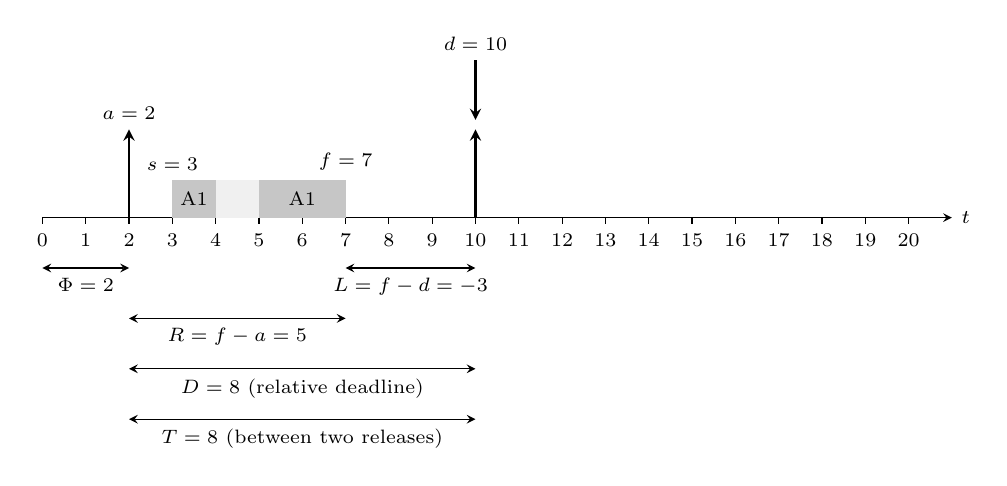
\begin{tikzpicture}[x=0.55cm, y=0.8cm, >=stealth, font=\scriptsize]
    % axis
    \draw[->] (0,0) -- (21,0) node[right] {$t$};
    \foreach \t in {0,...,20} \draw (\t,0) -- (\t,-0.1) node[below] {\t};
    % execution
    \fill[gray!45] (3,0) rectangle (4,0.6);
    \fill[gray!12] (4,0) rectangle (5,0.6);
    \fill[gray!45] (5,0) rectangle (7,0.6);
    \node at (3.5,0.3) {A1};
    \node at (6,0.3) {A1};
    \node[above] at (3,0.6) {$s=3$};
    \node[above] at (7,0.6) {$f=7$};
    % releases and deadline
    \draw[->, thick] (2,0) -- (2,1.4) node[above] {$a=2$};
    \draw[->, thick] (10,0) -- (10,1.4);
    \draw[->, thick] (10,2.5) -- (10,1.55);
    \node[above] at (10,2.5) {$d=10$};
    % dimensions
    \draw[<->] (0,-0.8) -- node[below] {$\Phi=2$} (2,-0.8);
    \draw[<->] (7,-0.8) -- node[below] {$L=f-d=-3$} (10,-0.8);
    \draw[<->] (2,-1.6) -- node[below] {$R=f-a=5$} (7,-1.6);
    \draw[<->] (2,-2.4) -- node[below] {$D=8$ (relative deadline)} (10,-2.4);
    \draw[<->] (2,-3.2) -- node[below] {$T=8$ (between two releases)} (10,-3.2);
\end{tikzpicture}
\caption{Task A: phase $\Phi = 2$, period $T = 8$, $C = 3$ ($1 + 2$). Its first job is released at 2, is preempted once (light grey: another task runs), and finishes at 7, three units before its deadline 10. The next job is released at 10, then at 18, and so on.}
\end{figure}
For a task A, with jobs $A_1$, $A_2$, \dots\ ($A_k$ is job $k$):
\begin{itemize}
    \item \textbf{release} (arrival, activation) time $a$: the job becomes READY. Job $k$ is released at
    \[
    a = \Phi + (k-1) \times T
    \]
    \item \textbf{phase} $\Phi$: the release time of the first job; usually all tasks start at 0 ($\Phi = 0$ if not given), but some systems must start a task a bit later;
    \item \textbf{computation time} $C$: the CPU time the job actually uses, taken in its worst case, the \textbf{WCET} (in the figure, A runs 1 unit and then 2, because another task runs in between: $C = 3$);
    \item \textbf{period} $T$, the time between two releases; \textbf{relative deadline} $D$, the time the job has after its release ($D = T$ here); \textbf{absolute deadline} $d = a + D$, the instant by which the job must be finished (with $D = T$, the next release);
    \item \textbf{start time} $s$ and \textbf{finish time} $f$; careful: in general $f \neq s + C$, because the job can be preempted (in the figure, $s + C = 6$ but $f = 7$);
    \item \textbf{response time} $R = f - a$, from release to end (in the figure, $7 - 2 = 5$); a job meets its deadline when $R \le D$;
    \item \textbf{lateness} $L = f - d$: negative = early, 0 = just in time, positive = deadline missed (in the figure, $7 - 10 = -3$). In a hard real-time system every job must always have $L \le 0$.
\end{itemize}
Unit 1 called $f - a$ the \emph{turnaround time} and $s - a$ the \emph{response time}; real-time systems call $f - a$ the response time, and from here on ``response time'' means $f - a$.

\subsection{Utilisation}
Periodic task sets can be analysed mathematically, and the first metric needed is the \textbf{utilisation factor}. A task needs $C$ units of CPU in each period $T$, so it uses the fraction $C/T$ of the CPU, its execution time normalised to its period (between 0 and 1); for a task set:
    \[
    U = \frac{C_1}{T_1} + \frac{C_2}{T_2} + \dots + \frac{C_n}{T_n} = \sum_{i=1}^{n} \frac{C_i}{T_i}
    \]
\begin{itemize}
    \item $U > 1$: the tasks need more CPU time than exists, and no algorithm can meet all deadlines on one CPU: the task set cannot be scheduled.
    \item $U \le 1$ is \textbf{necessary but not sufficient}: the set can potentially be scheduled, but an algorithm may still miss deadlines (examples with timeline scheduling, below). It would be sufficient only for a \emph{perfect} algorithm, able to use the CPU at 100\%: one exists, and will be studied, but it is complex, so in practice simpler schedulers are often preferred, paying for simplicity with non-optimality: they may fail even with $U \le 1$, \textbf{under-utilising} the CPU.
\end{itemize}
\textbf{In practice, check $U$ first}, even without knowing the algorithm: with $U > 1$, drawing a Gantt chart or applying an algorithm is a waste of time. At the exam, if $U > 1$, the following questions about the schedule need no answer: the problem cannot be solved.

\paragraph{In real life: what if $U > 1$?} The customer's product must schedule tasks with known execution times, periods and deadlines, and $U > 1$. In each ratio $C/T$, the \textbf{period} comes from the requirements and cannot change (e.g.\ the airbag must react within 1\,ms); the \textbf{computation time} can be reduced with better (more efficient) software, but only up to a limit, beyond which even the best possible designer cannot make the code faster. The usual solution is to \textbf{buy a faster CPU}: cost is important in embedded systems, so the design starts with a cheap CPU (e.g.\ an Arduino-class microcontroller costing a few euros) and, if the tasks do not fit, moves to a slightly more powerful CPU that costs more but fits them.

\subsection{Hyperperiod}
Each periodic task repeats with its own period, and the activations of all the tasks together repeat too, with period the \textbf{hyperperiod} $H$, the \textbf{least common multiple} (LCM) of the periods:
\[
H = \mathrm{LCM}(T_1, T_2, \dots, T_n)
\]
With all phases 0, every task releases a job at 0 and again at $H$, so it is enough to draw the schedule from 0 to $H$, in which task $i$ has exactly $H / T_i$ jobs. \textbf{Example}: A ($C = 2, T = 5$), B ($C = 2, T = 10$), C ($C = 2, T = 20$):
\[
U = \frac{2}{5} + \frac{2}{10} + \frac{2}{20} = \frac{8}{20} + \frac{4}{20} + \frac{2}{20} = \frac{14}{20} = \frac{7}{10} = 0.700
\]
The CPU is busy 70\% of the time.
\[
H = \mathrm{LCM}(5, 10, 20) = 20
\]
Whatever the schedule of the three tasks, it repeats every 20 time units: in each hyperperiod, A has 4 jobs, B has 2, C has 1.

\paragraph{Two ways to check schedulability.} \textbf{Mathematically}, for the algorithms of this course that come with a mathematical foundation (in practice, a formula to apply); or \textbf{empirically}, the only option for algorithms without a mathematical test: apply the algorithm and draw the Gantt chart on paper for one hyperperiod, since an algorithm that meets all deadlines in $[0, H)$ will always meet them.

\subsection{Why the worst-case execution time?}
\begin{lstlisting}[language=C]
void task_control( void )                /* one job */
{
    read_sensors();                      /* always:          40 us */
    if ( new_target_received() )         /* only sometimes:       */
        recompute_trajectory();          /*                 300 us */
    if ( error_detected() )              /* rarely:               */
        log_error_to_flash();            /*                 900 us */
    write_actuators();                   /* always:          20 us */
}
/* usually 60 us; worst case 40 + 300 + 900 + 20 = 1260 us */
\end{lstlisting}
A task has several execution paths, chosen by its input, each with its own time, and caches add more variation. A guarantee must hold for every job, so it uses the \textbf{WCET}, the longest time over all inputs and states: planning with the average (say 100\,$\mu s$), the rare job that takes 1260\,$\mu s$ would miss its deadline exactly when an error occurs.

\paragraph{Estimating the WCET is hard.} Some researchers have worked on it for 30 years: which side of a branch is taken depends on the values of variables, and therefore on the program's inputs, so for a complex program (say, a million assembly instructions) finding the path with the longest execution time \textbf{cannot be solved exactly}. In general, the WCET comes from measuring the longest run plus a margin, or from analysing the code: safe but pessimistic. The practical solution is \textbf{statistical}: run the program many times with different inputs, measure each execution time, build the distribution (the probability of each execution time) and estimate the WCET from it; but the inputs are usually random, and it is not known whether they are representative of the real application, so much research aims at better estimates. In this course the WCET is always \textbf{given}, but for an engineer designing a car's braking system computing it is a real problem, and when safety really matters it is \textbf{overestimated}: a measured execution time around 10 becomes 30 or 40 (three or four times larger), to be sure no deadline is missed. The price of overestimating is \textbf{wasted CPU time}.

\subsection{Exercise: notation}
A typical exercise gives a set of tasks with their periods and execution times; if nothing is said, all tasks are activated at time 0 ($\Phi = 0$). Three periodic tasks, all with phase 0 and $D = T$:
\begin{center}
\begin{tabular}{c c c}
\hline
task & $C$ & $T$ \\
\hline
A & 2 & 4 \\
B & 1 & 8 \\
C & 1 & 12 \\
\hline
\end{tabular}
\end{center}
\begin{enumerate}
    \item Compute $U$, as a fraction and with three decimals.
    \item Compute the hyperperiod $H$. How many jobs of each task are released in $[0, H)$?
    \item Job $B_2$ starts at 10 and finishes at 11. Compute its $a$, $d$, $R$ and $L$.
    \item Job $C_2$ starts at 14 and finishes at 15. Compute its $a$, $d$, $R$ and $L$.
    \item If C had phase $\Phi = 3$ instead, when would $C_2$ be released, and what would its absolute deadline be?
\end{enumerate}

\paragraph{Solution.}
\begin{enumerate}
    \item $U = \dfrac{2}{4} + \dfrac{1}{8} + \dfrac{1}{12} = \dfrac{12}{24} + \dfrac{3}{24} + \dfrac{2}{24} = \dfrac{17}{24} = 0.708$
    \item $H = \mathrm{LCM}(4, 8, 12) = 24$. Jobs in $[0, 24)$: A $24/4 = 6$, B $24/8 = 3$, C $24/12 = 2$.
    \item $B_2$: $a = 0 + 1 \times 8 = 8$, \quad $d = 8 + 8 = 16$, \quad $R = 11 - 8 = 3$, \quad $L = 11 - 16 = -5$.
    \item $C_2$: $a = 0 + 1 \times 12 = 12$, \quad $d = 12 + 12 = 24$, \quad $R = 15 - 12 = 3$, \quad $L = 15 - 24 = -9$.
    \item With $\Phi = 3$: $C_2$ is released at $a = 3 + 1 \times 12 = 15$, and its absolute deadline is $d = 15 + 12 = 27$.
\end{enumerate}
The start and finish times come from this schedule, built with the timeline method (next section). Both jobs finish early: negative lateness.
\begin{verbatim}
time  0         10        20
      |.........|.........|...
A     ##..##..##..##..##..##..
B     ..#.......#.......#.....
C     ...#..........#.........
CPU   AABCAA..AAB.AAC.AAB.AA..
\end{verbatim}

\section{Timeline scheduling}
The first real-time algorithm we study, \textbf{timeline scheduling} (or \textbf{cyclic executive}), is the worst in terms of efficiency: definitely not optimal, and without a mathematical foundation to check whether a task set can be scheduled (the only way is to try to build the Gantt chart). But it is very simple to implement, and used in many real products.

\subsection{The idea and the rules}
It suits simple embedded applications, a few periodic tasks that do not interact (e.g.\ reading sensors through one shared ADC and updating outputs), which do not need a full operating system.
\begin{itemize}
    \item The whole schedule is computed \textbf{offline}, before the system runs: the algorithm is applied on paper to decide the order and the activation time of every job, and the result is encoded as a fixed table. At run time no scheduler decides anything: the program follows the table (``this task starts at 0 and finishes here, then the next one runs, then the next one'').
    \item The time axis is divided into slots of equal length, the \textbf{minor cycles} (or \textbf{frames}): minor cycle $m$ $=$ the \textbf{greatest common divisor} (GCD) of the periods, so that every period is a whole number of frames and every release falls on a frame boundary. A timer interrupt marks the start of every frame, and each frame runs a fixed list of jobs, one after the other, without preemption.
    \item The \textbf{major cycle}, the sequence of frames that then repeats identically, is $M$ $=$ the LCM of the periods $=$ the \textbf{hyperperiod}: it is enough to fill the $M/m$ frames of one major cycle, and if all tasks fit, the schedule always repeats in the same way, starting again from frame 0.
\end{itemize}
The course rules to build the table:
\begin{itemize}
    \item Go through the frames in order. At the start of each frame, take the jobs already released and not yet run, and place them \textbf{shortest period first} (the most urgent task first; equal periods: lowest identifier first), each right after the previous one.
    \item A job is placed only if it \textbf{fits completely} in the time left in the frame: a job \textbf{cannot cross a frame boundary}. If it does not fit, it waits for a later frame, and the next jobs in the list are still tried.
    \item A placed job runs to the end without preemption; the rest of the frame is idle. Check per frame: the sum of the $C$ of its jobs is at most $m$.
    \item The table is \textbf{feasible} if every job is placed in a frame that ends by its deadline; a job that finds no such frame is a \textbf{deadline miss}.
\end{itemize}
The algorithm does not say \emph{where} in a frame a job goes (at the beginning, at the end, \dots): the course convention, used by \texttt{schedsim} and at the exam, is always the \textbf{first available slot}, so that every exercise has a single solution.

\subsection{Timeline: worked example}
The tasks of the hyperperiod example, all with the same execution time: A ($C = 2, T = 5$), B ($C = 2, T = 10$), C ($C = 2, T = 20$).
\[
U = \frac{7}{10} = 0.700, \qquad m = \mathrm{GCD}(5, 10, 20) = 5, \qquad M = \mathrm{LCM}(5, 10, 20) = 20
\]
Frames of 5 units; the hyperperiod is 20, so 4 frames are enough.
\begin{center}
\begin{tabular}{l l l l}
\hline
\textbf{frame} & \textbf{jobs} & \textbf{used} & \\
\hline
frame 0 $[0,5)$ & $A_1$ $B_1$ & 4/5 & $C_1$ does not fit (1 left): waits \\
frame 1 $[5,10)$ & $A_2$ $C_1$ & 4/5 & \\
frame 2 $[10,15)$ & $A_3$ $B_2$ & 4/5 & \\
frame 3 $[15,20)$ & $A_4$ & 2/5 & \\
\hline
\end{tabular}
\end{center}
\begin{verbatim}
time  0    5    10   15   20
      |....|....|....|....|
A     ##...##...##...##...
B     ..##........##......
C     .......##...........
CPU   AABB.AACC.AABB.AA...
\end{verbatim}
Intuitively, the most urgent task, A (period 5, equal to the minor cycle), gets one job in every frame, B one every two frames, and C one per major cycle, in the first frame where it fits without crossing a boundary. With the course rules: in frame 0 $[0,5)$, $A_1$, $B_1$ and $C_1$ are all released; shortest period first, $A_1$ (2 units, 3 left) and $B_1$ (2 units, 1 left) are placed, but $C_1$ needs 2 and would cross the frame boundary, so it waits. In frame 1 $[5,10)$, $A_2$ (released at 5, shorter period) goes before the waiting $C_1$: 4 units used. Frame 2 holds $A_3$ and $B_2$, released at 10; frame 3 only $A_4$. Every job is in a frame that ends by its deadline: the table is \textbf{feasible}, and $C_1$ (deadline 20) simply runs one frame after its release.

\paragraph{Why it is not optimal.} (From a question in class: what if the tasks had $C = 4$?) Longer execution times may give $U > 1$, which is impossible, but also $U < 1$ with a task set that still cannot be scheduled: the rule that forbids crossing a frame boundary creates \textbf{holes} where the CPU is idle, and that idle time is wasted and can never be recovered. Timeline scheduling is a perfect example of a non-optimal algorithm, for which $U \le 1$ is not enough (examples later in this section).

\subsection{How a cyclic executive is implemented}
The implementation is super simple: the scheduler is basically an infinite loop, with one function per minor cycle (four here) that calls the tasks of its frame in the order of the table:
\begin{lstlisting}[language=C]
/* A (C=2, T=5), B (C=2, T=10), C (C=2, T=20): each task is a function that runs one job */
static void frame_0( void ) { task_a(); task_b(); }    /* one function per minor cycle */
static void frame_1( void ) { task_a(); task_c(); }
static void frame_2( void ) { task_a(); task_b(); }
static void frame_3( void ) { task_a(); }

static volatile int frame_start;            /* set by the interrupt: volatile = re-read every time */

void SysTick_Handler( void ) { frame_start = 1; }      /* timer: every minor cycle (5 ms) */

static void wait_frame( void )              /* idle until the next frame boundary */
{
    while ( frame_start == 0 ) { }
    frame_start = 0;
}

int main( void )
{
    timer_start_ms( 5 );                    /* program the timer to the minor cycle (not shown) */
    for ( ;; )                              /* one turn of this loop = one major cycle (20 ms) */
    {
        wait_frame(); frame_0();
        wait_frame(); frame_1();
        wait_frame(); frame_2();
        wait_frame(); frame_3();
    }
}
\end{lstlisting}
\begin{itemize}
    \item Each task is a plain function that runs one job and returns; the major cycle is an endless loop that calls the frame functions in order.
    \item The timer fires once per minor cycle, and \texttt{wait\_frame} waits for it: when the jobs of a frame finish early, the loop waits for the beginning of the next frame, so each frame starts exactly on its boundary. \texttt{frame\_start} is \texttt{volatile} because the interrupt changes it: without \texttt{volatile}, the compiler could read it once and loop forever on the old value.
    \item No context switch, no TCB, no ready queue: all tasks run on one stack, inside one loop.
    \item If a frame overruns (its jobs take longer than $m$), the flag is already set when \texttt{wait\_frame} is called: a robust executive checks this and reports the error.
    \item Changing a task's $C$ or $T$ means recomputing the table and rewriting the frame functions.
\end{itemize}
With the order fixed on paper and always repeated, this scheduler is \textbf{extremely predictable}: this is why it is used in many safety-critical real-time applications, where certification needs a fixed, proven schedule, with periods chosen to fit it. In avionics basically every product uses it: aircraft fly with this algorithm, wasting CPU power but being super predictable. (The professor works on research contracts with automotive and avionics companies that are only now planning to introduce more advanced algorithms, in products that will reach the market in about ten years.)

\subsection{Timeline scheduling: pros and cons}
\begin{center}
\begin{tabular}{p{6.5cm} p{6.5cm}}
\hline
\textbf{pros} & \textbf{cons} \\
\hline
very simple: a loop, a timer, a table; no kernel needed & fragile: a new task or a changed $C$ or $T$ can change the whole table \\
very predictable: each job starts at a known time in its frame, with almost no variation & a job longer than a frame never fits: it must be split by hand \\
no preemption: no shared-data conflicts, no context-switch cost & aperiodic events must wait for a frame that checks for them (polling) \\
the schedule is checked offline, once, before the system runs & one job that overruns delays every following frame \\
 & non-harmonic periods give short frames and huge tables \\
\hline
\end{tabular}
\end{center}
Everything is checked offline, on paper, where the wasted CPU time is visible as idle slots: it is accepted in exchange for full predictability. \textbf{Fragility}: every control unit (ECU) in a car performs many activities, and a new task added by a firmware upgrade of the engine ECU can completely break the schedule. \textbf{Aperiodic events} are hard to fit efficiently in this mechanism. \textbf{Overruns}: the WCET is known in theory, but in practice there is always a small chance that a task runs longer than expected, and then the whole schedule is broken.

\subsection{Non-harmonic periods}
Everything looks perfect on paper when the periods are \textbf{harmonic}, i.e.\ each period divides every longer one, as in the example (5, 10, 20): then the GCD is the shortest period and the LCM the longest one. Periods that are not harmonic (e.g.\ chosen at random) cause \textbf{short frames}, because the GCD can be much smaller than every period (with $T = 5, 7, 11$ it is 1: a frame lasts one unit, and no job with $C \ge 2$ fits in any frame), and \textbf{huge tables}, because the LCM grows fast (with $T = 5, 7, 11$, $5 \times 7 \times 11 = 385$ frames to store, for three tasks: the system is still predictable, but the pattern repeats only after a long time). Two ways out:
\begin{itemize}
    \item \textbf{Split} a long task into parts that each fit in a frame (e.g.\ D with $C = 4$ becomes D with $C = 2$ and E with $C = 2$, same period). The parts must still run in order: give the first part the lower identifier, and check the order in the chart.
    \item \textbf{Shorten some periods} until they are harmonic: running a task more often than needed is always allowed, but $U$ grows. E.g.\ periods 2, 3 and 8 are not harmonic, but running the second task every 2 instead of every 3 gives 2, 2, 8, which are. This restricts the deadline of the second task: a CPU that could handle the original task set may no longer be enough, and a faster one is needed.
\end{itemize}
So timeline scheduling is simple, but far from perfect: CPU time is wasted both in the idle holes and in artificially shortened periods.

\paragraph{Example.} A ($C = 1, T = 4$) and B ($C = 3, T = 6$): $U = 1/4 + 3/6 = 0.750$; GCD $= 2$, LCM $= 12$. \textbf{As given}, frames of 2 units: schedule \texttt{A...A...A...}, because B needs 3 units but a frame has 2, so B \textbf{never fits}, and $B_1$ misses its deadline at 6: \textbf{not feasible}, even though $U$ is only 0.75. \textbf{With B's period shortened to 4}, the periods are harmonic, GCD $=$ LCM $= 4$: one frame, \texttt{ABBB}, \textbf{feasible}; B now runs every 4 instead of every 6 units, and $U = 1/4 + 3/4 = 1$: the CPU is never idle.

\subsection{Exercise: timeline scheduling}
Four periodic tasks, phase 0, $D = T$: A ($C = 1, T = 4$), B ($C = 2, T = 8$), C ($C = 1, T = 8$), D ($C = 2, T = 16$).
\begin{enumerate}
    \item Compute $U$, the minor cycle and the major cycle.
    \item Fill the frames with the course rules; in each frame, write the jobs and the time used.
    \item Draw the Gantt chart and write the schedule string. Is the timeline feasible?
    \item Compute $R$ and $L$ of job $D_1$.
\end{enumerate}

\textbf{Solution.}
\[
U = \frac{1}{4} + \frac{2}{8} + \frac{1}{8} + \frac{2}{16} = \frac{4}{16} + \frac{4}{16} + \frac{2}{16} + \frac{2}{16} = \frac{12}{16} = \frac{3}{4} = 0.750
\]
Minor cycle $= \mathrm{GCD}(4, 8, 8, 16) = 4$; major cycle $= \mathrm{LCM}(4, 8, 8, 16) = 16$: 4 frames.
\begin{center}
    \begin{tabular}{l l l l}
        \hline
        frame 0 $[0,4)$ & $A_1$ $B_1$ $C_1$ & 4/4 & $D_1$ does not fit (0 left): waits \\
        frame 1 $[4,8)$ & $A_2$ $D_1$ & 3/4 & \\
        frame 2 $[8,12)$ & $A_3$ $B_2$ $C_2$ & 4/4 & \\
        frame 3 $[12,16)$ & $A_4$ & 1/4 & \\
        \hline
    \end{tabular}
\end{center}
\begin{verbatim}
    time  0         10
        |.........|.....
    A     #...#...#...#...
    B     .##......##.....
    C     ...#.......#....
    D     .....##.........
    CPU   ABBCADD.ABBCA...
\end{verbatim}
\textbf{Feasible}. In frame 0 all four jobs are released; B and C have the same period, so B goes first (lowest identifier): $A_1$, $B_1$, $C_1$ fill the 4 units, and $D_1$ waits. In frame 1, $A_2$ (released at 4) goes before $D_1$ (shorter period), and $D_1$ runs from 5 to 7. $B_2$ and $C_2$ are released at 8, in frame 2. $D_1$: $a = 0$, $s = 5$, $f = 7$, $d = 16$; \quad $R = 7 - 0 = 7$, \quad $L = 7 - 16 = -9$.

\subsection{Exercise: a frame too small}
Four periodic tasks, phase 0, $D = T$: A ($C = 2, T = 6$), B ($C = 3, T = 12$), C ($C = 2, T = 12$), D ($C = 4, T = 24$).
\begin{enumerate}
    \item Compute $U$, the minor cycle and the major cycle. Does $U$ allow a feasible schedule?
    \item Fill the frames, draw the Gantt chart and write the schedule string. Is the timeline feasible? If not, which job misses, and when?
    \item Split D into two parts, D ($C = 2$) and E ($C = 2$), both with $T = 24$. Build the new table. Is it feasible, and do D and E run in the right order?
\end{enumerate}

\textbf{Solution (1, 2).}
\[
U = \frac{2}{6} + \frac{3}{12} + \frac{2}{12} + \frac{4}{24} = \frac{8}{24} + \frac{6}{24} + \frac{4}{24} + \frac{4}{24} = \frac{22}{24} = \frac{11}{12} = 0.917 \ (\le 1)
\]
Minor cycle $= \mathrm{GCD}(6, 12, 12, 24) = 6$; major cycle $= \mathrm{LCM}(6, 12, 12, 24) = 24$: 4 frames.
\begin{center}
    \begin{tabular}{l l l p{5.5cm}}
        \hline
        frame 0 $[0,6)$ & $A_1$ $B_1$ & 5/6 & $C_1$ (2) and $D_1$ (4) do not fit in 1 \\
        frame 1 $[6,12)$ & $A_2$ $C_1$ & 4/6 & $D_1$ (4) does not fit in 2 \\
        frame 2 $[12,18)$ & $A_3$ $B_2$ & 5/6 & $C_2$ and $D_1$ do not fit in 1 \\
        frame 3 $[18,24)$ & $A_4$ $C_2$ & 4/6 & $D_1$ (4) does not fit in 2: no frame left before 24 \\
        \hline
    \end{tabular}
\end{center}
\begin{verbatim}
    time  0         10        20
        |.........|.........|...
    A     ##....##....##....##....
    B     ..###.........###.......
    C     ........##..........##..
    D     ........................   <- D1 misses its deadline at 24
    CPU   AABBB.AACC..AABBB.AACC..
\end{verbatim}
\textbf{Not feasible}: $D_1$ misses its deadline at 24. There are 6 idle units in total, but never 4 in one frame.

\textbf{Solution (3).} Splitting does not change $U$: $U = 2/6 + 3/12 + 2/12 + 2/24 + 2/24 = 22/24 = 11/12 = 0.917$.
\begin{center}
    \begin{tabular}{l l l l}
        \hline
        frame 0 $[0,6)$ & $A_1$ $B_1$ & 5/6 & \\
        frame 1 $[6,12)$ & $A_2$ $C_1$ $D_1$ & 6/6 & $D_1$ (2) now fits in the 2 units left \\
        frame 2 $[12,18)$ & $A_3$ $B_2$ & 5/6 & \\
        frame 3 $[18,24)$ & $A_4$ $C_2$ $E_1$ & 6/6 & $E_1$ finishes at 24 $=$ its deadline: $L = 0$ \\
        \hline
    \end{tabular}
\end{center}
\begin{verbatim}
    time  0         10        20
        |.........|.........|...
    A     ##....##....##....##....
    B     ..###.........###.......
    C     ........##..........##..
    D     ..........##............
    E     ......................##
    CPU   AABBB.AACCDDAABBB.AACCEE
\end{verbatim}
\textbf{Feasible}. D (first part) runs at 10--12, E (second part) at 22--24: the order is right. In frame 0, $D_1$ and $E_1$ do not fit in the 1 unit left; in frame 2, $C_2$ and $E_1$ do not fit either; so $E_1$ runs only in frame 3. The CPU is idle only 2 units in 24.

\section{A tool to check your schedules: schedsim}
The way to learn the many scheduling algorithms is to do many exercises, possibly inventing new ones; and since everything in scheduling is an algorithm, the solution of any exercise can be automated. The course provides \textbf{schedsim} (in \texttt{course-material/tools/schedsim/}), a small Python program that implements all the scheduling algorithms of the course and follows exactly the rules and tie rules of this week: use it after solving on paper, not instead. It is plain Python 3: it runs with \texttt{python3}, nothing to install. The \textbf{input} is a small text file with the task set, in the slide notation: the algorithm to apply, followed by the data that algorithm needs (different for each algorithm); the folder \texttt{examples/} contains one example file per algorithm.
\begin{itemize}
    \item \texttt{explain <file>} solves the exercise and explains every single step, as the solution should be written at the exam ($U$, the frames, the chart, each job's times, every decision); \texttt{solve <file>} gives only the official answers, in the answer format.
    \item \texttt{check <file> <answers>} marks an answer file and, for a wrong schedule, says the first wrong slot and the rule that decides it.
    \item \texttt{run <file>} draws only the Gantt chart; \texttt{generate timeline --seed N} creates a new practice exercise (the same seed always gives the same one).
\end{itemize}

\subsection{Try it: explain, solve and check a timeline}
The task-set file \texttt{examples/timeline.txt}, and its explanation:
\begin{lstlisting}
    algorithm: timeline
    task A C=2 T=5
    task B C=2 T=10
    task C C=2 T=20
\end{lstlisting}
\begin{lstlisting}[language=bash]
    cd course-material/tools/schedsim
    python3 schedsim.py explain examples/timeline.txt
\end{lstlisting}
Output (excerpt; the full output also lists every job and every decision):
\begin{verbatim}
    == Timeline analysis ==
    U = sum C/T = 2/5 + 2/10 + 2/20 = 7/10 = 0.700
    minor cycle = GCD of periods = 5, major cycle = LCM of periods = 20
    frame 0 [0,5): A1 B1 (4/5 used)
    frame 1 [5,10): A2 C1 (4/5 used)
    frame 2 [10,15): A3 B2 (4/5 used)
    frame 3 [15,20): A4 (2/5 used)
    every job fits in a frame: the timeline is feasible
    == Schedule ==
    time  0    5    10   15   20
        |....|....|....|....|
    A     ##...##...##...##...
    B     ..##........##......
    C     .......##...........
    CPU   AABB.AACC.AABB.AA...
    schedule=AABB.AACC.AABB.AA...
    job  release  start  finish  deadline  response  lateness
    C1   0        7      9       20        9         -11
\end{verbatim}
\texttt{\#} $=$ the task runs in that slot; response is $R = f - a$, lateness is $L = f - d$. Then \texttt{solve}, and \texttt{check} on answers whose schedule contains one mistake:
\begin{lstlisting}[language=bash]
    python3 schedsim.py solve examples/timeline.txt
    printf 'schedule=AABB.AACC.AABB.AAC..\nU=7/10\nfeasible=yes\nfirst_miss=none\n' \
    | python3 schedsim.py check examples/timeline.txt -
\end{lstlisting}
The \verb|\| continues the command on the next line; the \texttt{-} tells \texttt{check} to read the answers from its standard input (normally they are written in a file, e.g.\ \texttt{my.txt}, checked with \texttt{check examples/timeline.txt my.txt}).
\begin{verbatim}
    $ python3 schedsim.py solve examples/timeline.txt
    schedule=AABB.AACC.AABB.AA...
    U=0.700
    feasible=yes
    first_miss=none

    $ printf '...' | python3 schedsim.py check examples/timeline.txt -
    schedule: WRONG
    first difference at slot 17: expected ., given C
    why: t=17: nothing planned in this part of the frame, idle
    U: correct
    feasible: correct
    first_miss: correct
    score: 3/4
\end{verbatim}
Slot 17 is in frame 3, which holds only $A_4$: C has one job per major cycle, already run in frame 1. \texttt{U=7/10} is marked correct although the solution says \texttt{0.700}: both forms are accepted.

\subsection{The answer format}
The same format is used by the tool and in the \textbf{written exam} (rules in \texttt{Exam.md}, section ``Scheduling exercises: conventions and answer format''):
\begin{itemize}
    \item One answer per line, as \texttt{key=value}, no spaces.
    \item \texttt{schedule=} then one character per time unit: the identifier of the task that runs, or \texttt{.} when the CPU is idle; a 20-unit schedule has exactly 20 characters.
    \item \texttt{U=} as a fraction (\texttt{7/10}) or a decimal rounded to three places (\texttt{0.700}; $17/24 \to$ \texttt{0.708}). Any fractional value, not only \texttt{U}, may be written either way: for the first FCFS worked example, \texttt{avgW} is \texttt{11/3} or \texttt{3.667} (the slides round it to 3.67 to fit the table).
    \item \texttt{feasible=yes} or \texttt{feasible=no}; \texttt{first\_miss=} the first deadline missed, as \texttt{<task>@<time of the deadline>} (e.g.\ \texttt{B@6}, or \texttt{D@24} in the ``frame too small'' exercise), or \texttt{none}.
    \item \texttt{R\_<id>} and \texttt{L\_<id>} for the response time and lateness of a job when an exercise asks for them, e.g.\ \texttt{R\_D1=7}, \texttt{L\_D1=-9}. For a timeline, \texttt{check} marks only \texttt{schedule}, \texttt{U}, \texttt{feasible} and \texttt{first\_miss}.
    \item For the algorithms of Unit 1 (FCFS, round robin, priority), the keys are \texttt{W\_<id>} (waiting time), \texttt{TA\_<id>} (turnaround time), \texttt{avgW} and \texttt{avgTA}.
    \item The scheduling conventions (time in whole units, $D = T$, the tie rules, higher number = higher priority) are those of \texttt{Exam.md}: the same in the slides, the tool and the exam.
\end{itemize}
For example, \texttt{solve} on the FCFS exercise of Unit 1 (the file \texttt{course-material/images/week-05/w5-fcfs-try.txt}) prints:
\begin{verbatim}
    schedule=AAAABBBC.DD
    W_A=0
    W_B=2
    W_C=4
    W_D=0
    TA_A=4
    TA_B=5
    TA_C=5
    TA_D=2
    avgW=1.500
    avgTA=4
\end{verbatim}

\paragraph{Why use the tool.} It is a good way to practise, since you can invent as many exercises as you want and get their solutions, and it makes you familiar with the \textbf{answer format}. At the exam the scheduling exercises are a pre-formatted text file where the answers must be filled in, and the professor grades them by running \texttt{schedsim check} on them. The format must be respected: if it is broken, the tool marks the exercise as wrong even if the solution is correct. In that case the exercise can be checked manually, on request by email, but with about 360 students at the exam, respecting the format is what makes automatic grading possible.

\section{Unit 3: summary}
\begin{itemize}
    \item A real-time system must be correct and on time: the right result after the deadline is a failure. Real-time is not fast: it guarantees each task, not the average.
    \item Deadlines are hard (a miss is catastrophic), firm (a late result is useless) or soft (a late result is still useful).
    \item Tasks are periodic (every $T$), sporadic (a minimum gap between jobs) or aperiodic (no known gap).
    \item Notation: release $a$, phase $\Phi$, WCET $C$, period $T$, relative deadline $D = T$, absolute deadline $d = a + D$, response time $R = f - a$, lateness $L = f - d$.
    \item Utilisation $U = \sum C/T$ must be at most 1; the hyperperiod is the LCM of the periods. We plan with the WCET, never the average.
    \item Timeline scheduling: minor cycle $=$ GCD, major cycle $=$ LCM, jobs placed shortest period first into frames, no preemption; simple and predictable but fragile, and non-harmonic periods make it fail or explode.
    \item \texttt{schedsim} (\texttt{explain}, \texttt{solve}, \texttt{check}) checks paper solutions, with the answer format and conventions of the exam.
\end{itemize}


\section{A prova di coglione}
Fino alla settimana scorsa lo scratch-OS eseguiva i task \emph{uno dopo l'altro}. Questo capitolo risponde a una domanda: come si fa a far girare più task ``insieme'' su una sola CPU e, quando serve, a garantire che ognuno finisca \emph{in tempo}? Il percorso è diviso in tre unità.

\begin{itemize}
    \item \textbf{Unità 1: le idee (solo teoria).} Che cos'è un task e in quali stati si trova (pronto, in esecuzione, bloccato, terminato); che cosa il kernel deve ricordare di ognuno (il TCB); quando entra in gioco lo scheduler. Poi tre politiche per decidere chi usa la CPU: \emph{first-come first-served}, \emph{round robin} e \emph{priorità}. Si confrontano con semplici misure (tempi di attesa, di risposta, di completamento) su esercizi svolti a mano, con le regole che valgono anche all'esame.
    \item \textbf{Unità 2: lo scratch-OS diventa multitasking.} Si studia il codice che realizza il round robin: il \emph{context switch} (salvare un task e riprenderne un altro esattamente da dove si era fermato), fatto con l'eccezione PendSV; il tick di sistema che scandisce i turni; le chiamate che cedono la CPU (yield, delay); il task \emph{idle}, che gira quando nessun altro può. Alla fine si scrive un piccolo \emph{trace} che mostra chi ha usato la CPU e quando. È la base del progetto del corso.
    \item \textbf{Unità 3: il tempo reale.} Nei sistemi real-time conta arrivare \emph{in tempo}, non essere veloci in media. Si classificano le scadenze (hard, firm, soft) e i task (periodici, sporadici, aperiodici), si introducono le grandezze per ragionarci (utilizzo della CPU, iperperiodo, tempo di esecuzione nel caso peggiore) e un primo metodo per pianificare tutto in anticipo, il \emph{timeline scheduling}. Lo strumento \texttt{schedsim} permette di controllare le soluzioni nel formato richiesto all'esame.
\end{itemize}

In breve: prima \emph{che cosa} significa schedulare, poi \emph{come} lo fa davvero un sistema operativo, infine \emph{quando} non basta essere veloci ma bisogna essere puntuali.


\subsection{Unità 1}

\subsection{Unità 2}

\subsection{Unità 3}
